\chapter{Resultados}

\begin{table}[htbp]
\centering
\caption{Tabla descriptiva de grupos de edad por intervalos de 6 meses}
\label{tab:grupos_edad_6meses}
\begin{threeparttable}
\begin{tblr}{
  width = \linewidth,
  colspec = {X[2,c]X[1,c]X[1,c]X[1,c]X[1,c]X[1,c]X[1,c]},
  row{1} = {font=\bfseries, bg=gray!10},
  row{even} = {bg=gray!3},
  row{Z} = {font=\bfseries, bg=gray!15},
  cells = {valign=m, font=\footnotesize},
  hline{1,2,Z} = {1pt},
  hline{3-Y} = {0.5pt, gray},
}
\textbf{Grupo de edad} & {\textbf{Femenino}\\(n)} & \textbf{Femenino (\%)} & {\textbf{Masculino}\\(n)} & \textbf{Masculino (\%)} & {\textbf{Total}\\(n)} & \textbf{Total (\%)} \\
0-6 & 134 & 16.7 & 129 & 14.0 & 263 & 15.2 \\
7-12 & 159 & 19.8 & 181 & 19.6 & 340 & 19.7 \\
13-18 & 105 & 13.1 & 117 & 12.7 & 222 & 12.9 \\
19-24 & 106 & 13.2 & 133 & 14.4 & 239 & 13.9 \\
25-30 & 72 & 9.0 & 90 & 9.8 & 162 & 9.4 \\
31-36 & 75 & 9.3 & 108 & 11.7 & 183 & 10.6 \\
37-42 & 35 & 4.4 & 54 & 5.9 & 89 & 5.2 \\
43-48 & 47 & 5.9 & 42 & 4.6 & 89 & 5.2 \\
49-54 & 38 & 4.7 & 41 & 4.4 & 79 & 4.6 \\
55-60 & 32 & 4.0 & 27 & 2.9 & 59 & 3.4 \\
\textbf{Total} & \textbf{803} & \textbf{100.0} & \textbf{922} & \textbf{100.0} & \textbf{1,725} & \textbf{100.0} \\
\end{tblr}
\begin{tablenotes}
\footnotesize
\item \textit{Nota:} Los grupos de edad están expresados en meses.
\end{tablenotes}
\end{threeparttable}
\end{table}

\begin{table}[htbp]
\centering
\caption{Distribución de niños de acuerdo a edad gestacional}
\label{tab:eg}
\begin{threeparttable}
\begin{tblr}{
  width = 0.8\linewidth,
  colspec = {X[2,l]X[1,c]X[1,c]},
  row{1} = {font=\bfseries, bg=gray!10},
  row{even} = {bg=gray!3},
  cells = {valign=m, font=\footnotesize},
  hline{1,2,Z} = {1pt},
  hline{3-Y} = {0.5pt, gray},
}
\textbf{Categoría} & \textbf{Cantidad} & \textbf{Porcentaje (\%)} \\
A término & 1,545 & 89.5 \\
Pretérmino tardío & 114 & 6.6 \\
Pretérmino moderado & 57 & 3.3 \\
Muy pretérmino & 9 & 0.5 \\
\textbf{Total} & \textbf{1,725} & \textbf{100.0} \\
\end{tblr}
\begin{tablenotes}
\footnotesize
\item \textit{Criterios de clasificación:} A término (37-42 semanas), Pretérmino tardío (34-36 semanas), Pretérmino moderado (32-33 semanas), Muy pretérmino ($<$32 semanas).
\end{tablenotes}
\end{threeparttable}
\end{table}

\begin{table}[htbp]
\centering
\caption{Distribución por etnia y área de residencia}
\label{tab:etnia-residencia}
\begin{threeparttable}
\begin{tblr}{
  width = \linewidth,
  colspec = {X[2,l]X[1,c]X[1,c]X[1,c]X[1,c]},
  row{1} = {font=\bfseries, bg=gray!10},
  row{even} = {bg=gray!3},
  cells = {valign=m, font=\footnotesize},
  hline{1,2,Z} = {1pt},
  hline{3-Y} = {0.5pt, gray},
}
\textbf{Etnia} & {\textbf{Área rural}\\n (\%)} & {\textbf{Área urbana}\\n (\%)} & {\textbf{Total}\\n (\%)} \\
Indígena & 183 (71.2) & 558 (38.0) & 741 (42.96) \\
No indígena & 74 (28.8) & 910 (62.0) & 984 (57.04) \\
\textbf{Total} & \textbf{257 (14.90)} & \textbf{1,468 (85.10)} & \textbf{1,725 (100.0)} \\
\end{tblr}
\begin{tablenotes}
\footnotesize
\end{tablenotes}
\end{threeparttable}
\end{table}

\begin{table}[htbp]
\centering
\caption{Distribución de edad materna y paterna}
\label{tab:edad_padres}
\begin{threeparttable}
\begin{tblr}{
  width = 0.9\linewidth,
  colspec = {X[2,c]X[1,c]X[1,c]X[1,c]X[1,c]},
  row{1} = {font=\bfseries, bg=gray!10},
  row{even} = {bg=gray!3},
  cells = {valign=m, font=\footnotesize},
  hline{1,2,Z} = {1pt},
  hline{3-Y} = {0.5pt, gray},
}
{\textbf{Intervalo de}\\    \textbf{Edad (años)}} & {\textbf{Madres}\\n} & {\textbf{Madres}\\    \textbf{(\%)}} & {\textbf{Padres}\\n} & {\textbf{Padres}\\    \textbf{(\%)}} \\
14-19 & 104 & 6.1 & 40 & 2.4 \\
20-24 & 412 & 24.0 & 304 & 18.2 \\
25-29 & 548 & 32.0 & 457 & 27.3 \\
30-34 & 433 & 25.3 & 430 & 25.7 \\
35-39 & 180 & 10.5 & 292 & 17.4 \\
40-44 & 31 & 1.8 & 106 & 6.3 \\
45+ & 6 & 0.4 & 45 & 2.7 \\
\textbf{Total}\tnote{a} & \textbf{1,714} & \textbf{100.0} & \textbf{1,674} & \textbf{100.0} \\
\end{tblr}
\begin{tablenotes}
\footnotesize
\item[a] Datos disponibles para 1,714 madres y 1,674 padres de la muestra total de 1,725 niños.
\item \textit{Estadísticas descriptivas:} Edad materna promedio: 27.85 años (DE: 5.59); Edad paterna promedio: 30.42 años (DE: 6.64).
\end{tablenotes}
\end{threeparttable}
\end{table}

\begin{table}[htbp]
\centering
\caption{Nivel educativo materno y paterno}
\label{tab:escolaridad}
\begin{threeparttable}
\begin{tblr}{
  width = 0.9\linewidth,
  colspec = {X[2,l]X[1,c]X[1,c]X[1,c]X[1,c]},
  row{1} = {font=\bfseries, bg=gray!10},
  row{even} = {bg=gray!3},
  cells = {valign=m, font=\footnotesize},
  hline{1,2,Z} = {1pt},
  hline{3-Y} = {0.5pt, gray},
}
\textbf{Nivel educativo} & {\textbf{Madre}\\n} & \textbf{Madre (\%)} & {\textbf{Padre}\\n} & \textbf{Padre (\%)} \\
Ninguna & 63 & 3.68 & 50 & 2.99 \\
Primaria & 315 & 18.38 & 259 & 15.49 \\
Básico & 507 & 29.58 & 380 & 22.73 \\
Diversificado & 701 & 40.90 & 811 & 48.50 \\
Universitario & 128 & 7.47 & 172 & 10.29 \\
\textbf{Total}\tnote{a} & \textbf{1,714} & \textbf{100.0} & \textbf{1,672} & \textbf{100.0} \\
\end{tblr}
\begin{tablenotes}
\footnotesize
\item[a] Datos disponibles para 1,714 madres y 1,672 padres de la muestra total.
\item \textit{Nota:} Los padres muestran mayor proporción de educación diversificada y universitaria comparado con las madres ($p < 0.05$).
\end{tablenotes}
\end{threeparttable}
\end{table}

\begin{table}[htbp]
\centering
\caption{Condición laboral materna y paterna}
\label{tab:empleo}
\begin{threeparttable}
\begin{tblr}{
  width = 0.9\linewidth,
  colspec = {X[2,l]X[1,c]X[1,c]X[1,c]X[1,c]},
  row{1} = {font=\bfseries, bg=gray!10},
  row{even} = {bg=gray!3},
  cells = {valign=m, font=\footnotesize},
  hline{1,2,Z} = {1pt},
  hline{3-Y} = {0.5pt, gray},
}
\textbf{Tipo de empleo} & {\textbf{Madre}\\n} & \textbf{Madre (\%)} & {\textbf{Padre}\\n} & \textbf{Padre (\%)} \\
Trabajo formal & 504 & 29.65 & 1,056 & 63.01 \\
Trabajo informal & 346 & 20.35 & 464 & 27.68 \\
No trabaja & 850 & 50.00 & 156 & 9.31 \\
\textbf{Total}\tnote{a} & \textbf{1,700} & \textbf{100.0} & \textbf{1,676} & \textbf{100.0} \\
\end{tblr}
\begin{tablenotes}
\footnotesize
\item[a] Datos disponibles para 1,700 madres y 1,676 padres con información laboral completa.
\item \textit{Nota:} Diferencias significativas en patrones de empleo por género ($p < 0.001$, prueba de chi-cuadrado).
\end{tablenotes}
\end{threeparttable}
\end{table}

\begin{table}[htbp]
\centering
\caption{Acceso a servicios básicos en el hogar}
\label{tab:servicios_basicos}
\begin{threeparttable}
\begin{tblr}{
  width = \linewidth,
  colspec = {X[3,l]X[2,l]X[1,c]X[1,c]},
  row{1} = {font=\bfseries, bg=gray!10},
  row{even} = {bg=gray!3},
  cells = {valign=m, font=\footnotesize},
  hline{1,2,Z} = {1pt},
  hline{3-Y} = {0.5pt, gray},
}
\textbf{Variable} & \textbf{Categoría} & \textbf{Frecuencia} & \textbf{Porcentaje (\%)} \\
\textbf{Agua para consumo del hogar} & Red de tubería & 1,562 & 90.55 \\
& Chorro público & 142 & 8.23 \\
& Pozo público o privado & 18 & 1.04 \\
& Río, lago, tonel, camión y otro & 3 & 0.17 \\
\textbf{Tipo de servicio sanitario} & Inodoro & 1,615 & 93.62 \\
& Letrina/Pozo ciego & 109 & 6.32 \\
& Excusado lavable & 1 & 0.06 \\
\textbf{Eliminación de basura} & Servicio municipal o privado & 1,482 & 85.91 \\
& La quema & 223 & 12.93 \\
& La tira en cualquier lugar & 9 & 0.52 \\
& La entierra & 8 & 0.46 \\
& Otra & 3 & 0.17 \\
\textbf{Tipo de alumbrado} & Eléctrico & 1,725 & 100.0 \\
\textbf{Fuente de energía para cocinar} & Gas propano & 1,503 & 87.13 \\
& Leña & 216 & 12.52 \\
& Gas corriente, carbón y otros & 4 & 0.23 \\
& Electricidad & 2 & 0.12 \\
\end{tblr}
\begin{tablenotes}
\footnotesize
\end{tablenotes}
\end{threeparttable}
\end{table}

\begin{table}[htbp]
\centering
\caption{Características de la composición familiar}
\label{tab:composicion_familiar}
\begin{threeparttable}
\begin{tblr}{
  width = \linewidth,
  colspec = {X[3,l]X[1,c]X[1,c]X[2,l]X[1,c]X[1,c]X[2,l]X[1,c]X[1,c]},
  row{1} = {font=\bfseries, bg=gray!10},
  row{even} = {bg=gray!3},
  cells = {valign=m, font=\scriptsize},
  hline{1,2,Z} = {1pt},
  hline{3-Y} = {0.5pt, gray},
}
{\textbf{Personas en}\\    \textbf{el hogar}} & \textbf{n} & \textbf{(\%)} & {\textbf{Número de}\\    \textbf{hermanos}} & \textbf{n} & \textbf{(\%)} & {\textbf{Posición}\\    \textbf{del niño}} & \textbf{n} & \textbf{(\%)} \\
1-2 & 1 & 0.06 & 0 & 540 & 31.3 & Primero & 694 & 40.23 \\
3-4 & 751 & 43.54 & 1 & 591 & 34.26 & Segundo & 616 & 35.71 \\
5-6 & 573 & 33.22 & 2 & 381 & 22.09 & Tercero & 372 & 21.57 \\
7-8 & 269 & 15.59 & 3 & 144 & 8.35 & Cuarto & 37 & 2.14 \\
9-10 & 68 & 3.94 & 4 & 47 & 2.72 & Quinto & 3 & 0.17 \\
11+ & 63 & 3.65 & 5 & 17 & 0.99 & Sexto & 2 & 0.12 \\
 & & & $\geq$6 & 5 & 0.29 & Séptimo+ & 1 & 0.06 \\
\textbf{Total} & \textbf{1,725} & \textbf{100.0} & \textbf{Total} & \textbf{1,725} & \textbf{100.0} & \textbf{Total} & \textbf{1,725} & \textbf{100.0} \\
\end{tblr}
\begin{tablenotes}
\footnotesize
\item \textit{Nota:} Promedio de personas por hogar: 5.32 (DE: 2.34); promedio de hermanos: 1.21 (DE: 1.15).
\end{tablenotes}
\end{threeparttable}
\end{table}

\begin{table}[htbp]
\centering
\caption{Acceso a cuidados prenatales}
\label{tab:cuidados_prenatales}
\begin{threeparttable}
\begin{tblr}{
  width = \linewidth,
  colspec = {X[2,l]X[1,c]X[1,c]X[3,l]X[1,c]X[1,c]},
  row{1} = {font=\bfseries, bg=gray!10},
  row{even} = {bg=gray!3},
  cells = {valign=m, font=\footnotesize},
  hline{1,2,Z} = {1pt},
  hline{3-Y} = {0.5pt, gray},
}
\textbf{Variable} & \textbf{Categoría} & \textbf{(\%)} & \textbf{Variable} & \textbf{Categoría} & \textbf{(\%)} \\
{\textbf{Controles}\\    \textbf{prenatales}} & 0 & 0.93 & {\textbf{Ultrasonido}\\    \textbf{obstétrico}} & No & 5.45 \\
& 1-2 & 4.46 & & Sí & 94.55 \\
& 3-4 & 22.49 & {\textbf{Vitaminas}\\    \textbf{(1er trimestre)}} & No & 11.83 \\
& 5-6 & 34.96 & & Sí & 88.17 \\
& 7-10 & 36.46 & {\textbf{Vitaminas}\\    \textbf{(resto embarazo)}} & No & 7.07 \\
& $\geq$11 & 0.70 & & Sí & 92.93 \\
\end{tblr}
\begin{tablenotes}
\footnotesize
\item \textit{Nota:} Promedio de controles prenatales: 6.70 (DE: 1.99).
\end{tablenotes}
\end{threeparttable}
\end{table}

\begin{figure}[htbp]
    \centering
    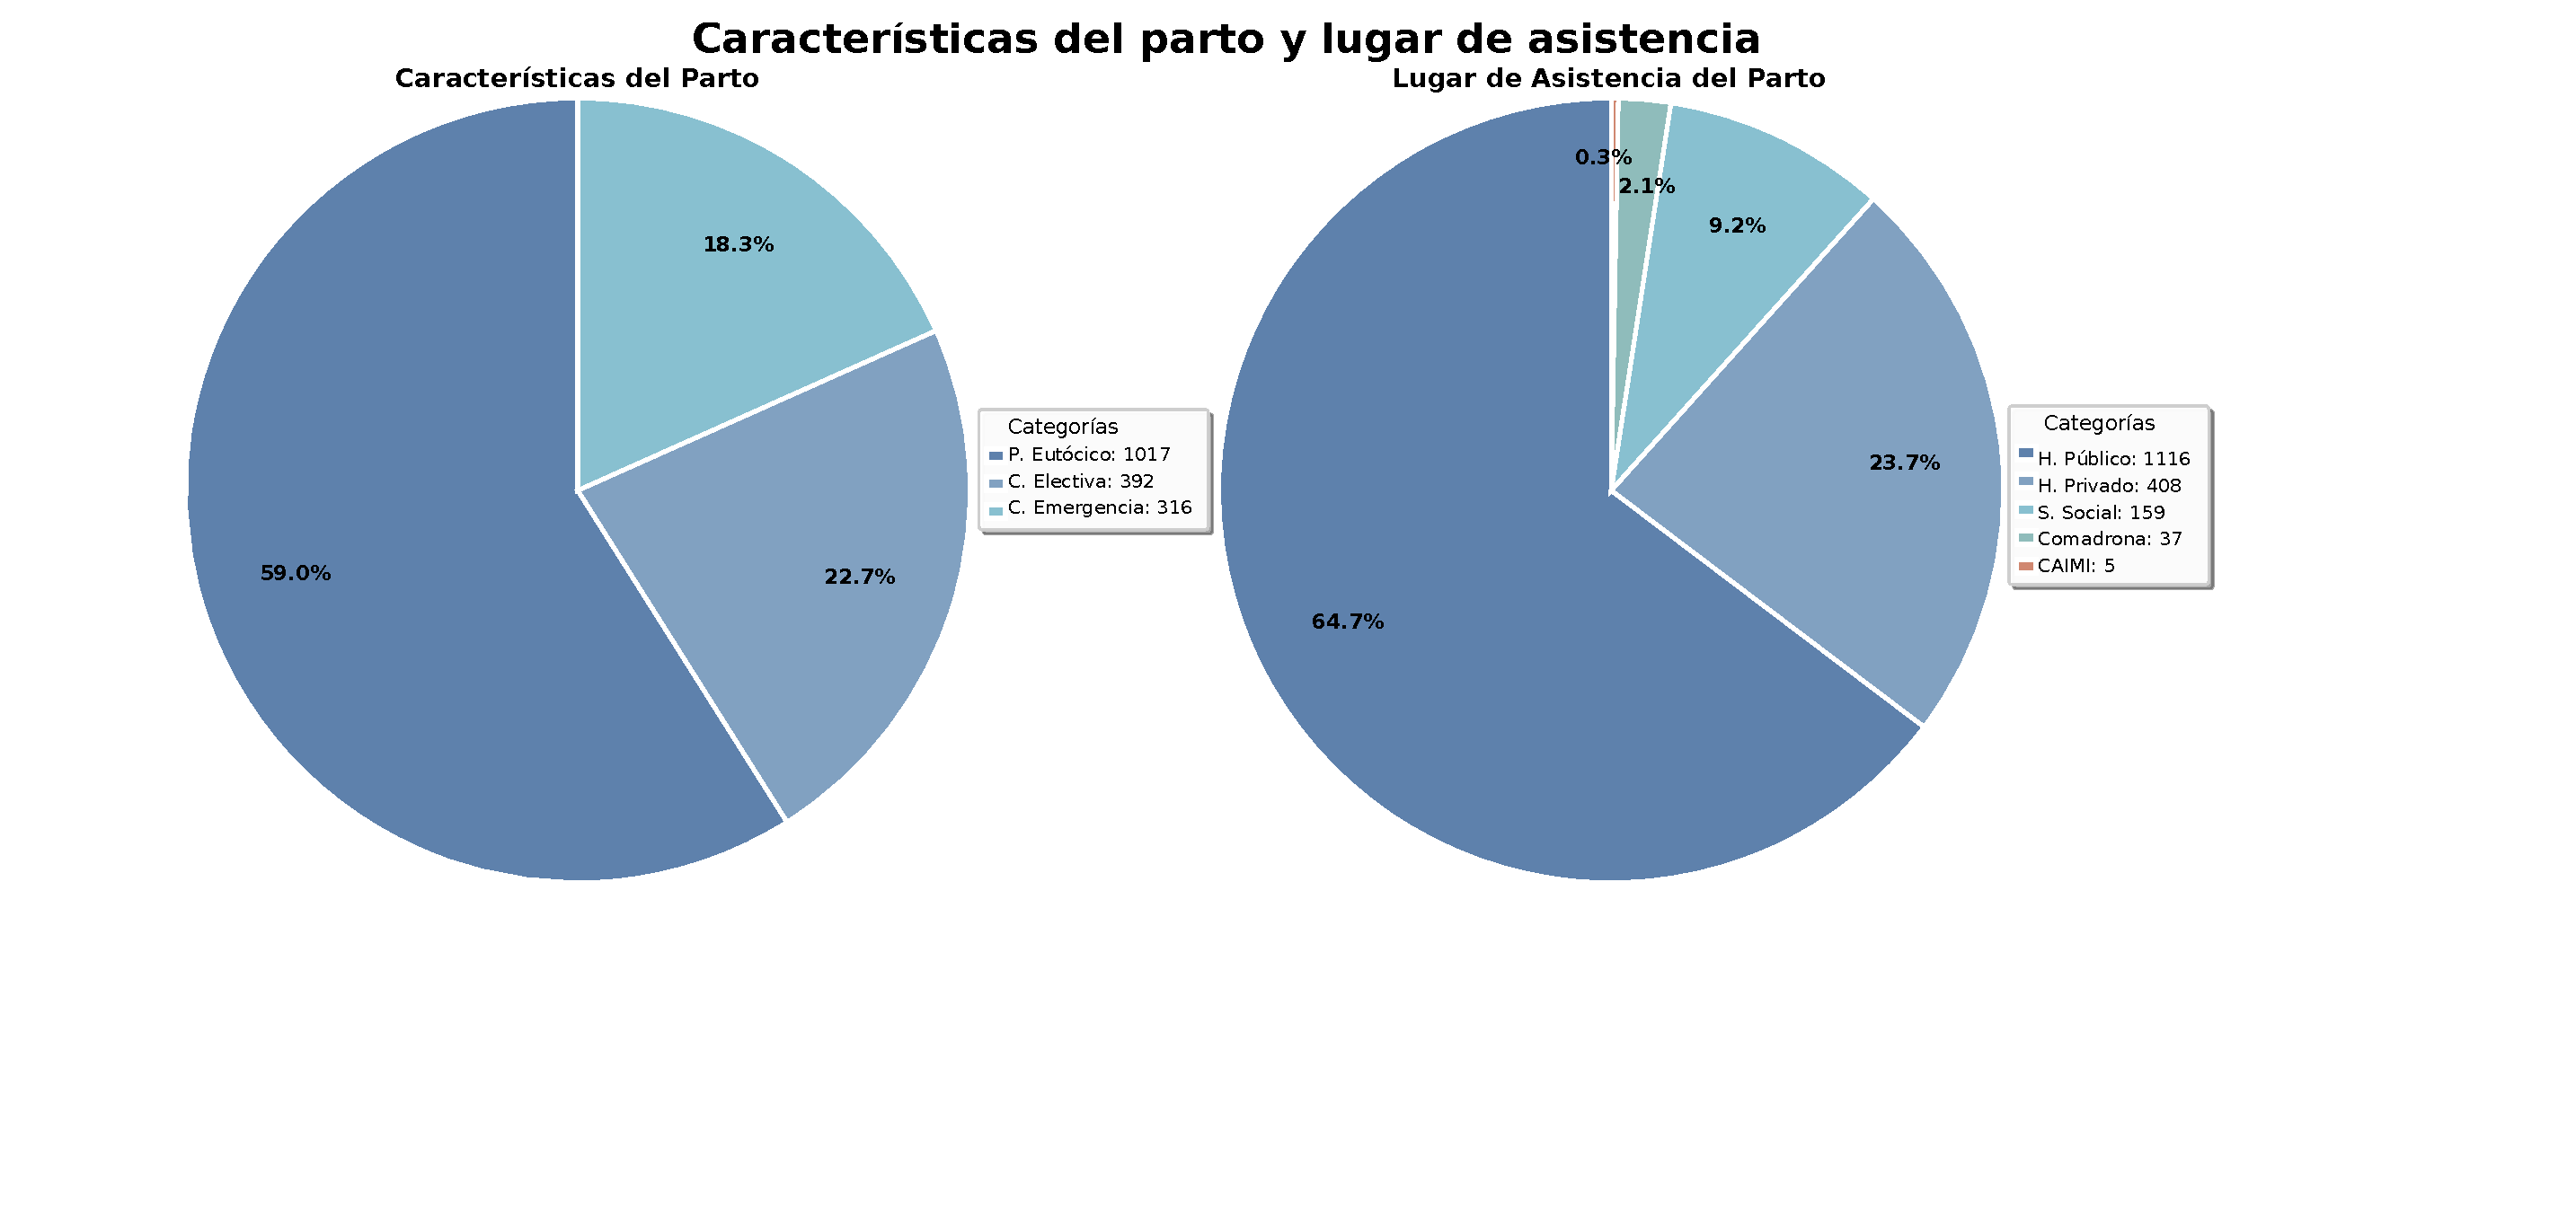
\includegraphics[width=1\textwidth]{grafica_asistencia_parto}
	\captionsetup{font=footnotesize}
    \caption{Distribución de lugar de asistencia y tipo de parto.}
    \label{fig:parto}
\end{figure}

\begin{table}[htbp]
\centering
\caption{Causas de césarea de emergencia}
\label{tab:causas_cesarea}
\begin{threeparttable}
\begin{tblr}{
  width = \linewidth,
  colspec = {X[4,l]X[1,c]X[1,c]},
  row{1} = {font=\bfseries, bg=gray!10},
  row{even} = {bg=gray!3},
  cells = {valign=m, font=\footnotesize},
  hline{1,2,Z} = {1pt},
  hline{3-Y} = {0.5pt, gray},
}
\textbf{Categoría} & \textbf{Frecuencia} & \textbf{Porcentaje} \\
Complicaciones del líquido amniótico & 138 & 43.4\% \\
Sufrimiento fetal & 84 & 26.4\% \\
Preeclampsia & 36 & 11.3\% \\
Falta de progresión del trabajo de parto & 23 & 7.2\% \\
Presentación fetal anómala & 11 & 3.5\% \\
Ruptura pretérmino de membranas ovulares & 5 & 1.6\% \\
Problemas de placenta & 3 & 0.9\% \\
Embarazo múltiple & 2 & 0.6\% \\
Infección materna & 1 & 0.3\% \\
Otras causas & 14 & 4.4\% \\
\textbf{Total} & \textbf{317} & \textbf{100.0\%} \\
\end{tblr}
\begin{tablenotes}
\footnotesize
\item \textit{Nota:} Datos de acuerdo a 317 casos de césarea de emergencia de un total de 1,725 nacimientos.
\end{tablenotes}
\end{threeparttable}
\end{table}

\begin{table}[htbp]
\centering
\caption{Patrones de lactancia durante los primeros 24 meses de vida}
\label{tab:lactancia_periodos}
\begin{threeparttable}
\begin{tblr}{
  width = \linewidth,
  colspec = {X[3,l]X[1,c]X[1,c]X[1,c]},
  row{1} = {font=\bfseries, bg=gray!10},
  row{even} = {bg=gray!3},
  cells = {valign=m, font=\footnotesize},
  hline{1,2,Z} = {1pt},
  hline{3-Y} = {0.5pt, gray},
}
\textbf{Tipo de lactancia} & {\textbf{0-6 meses}\\n (\%)} & {\textbf{6-12 meses}\\n (\%)} & {\textbf{12-24 meses}\\n (\%)} \\
Lactancia materna exclusiva & 1,254 (72.7) & 867 (55.6) & 609 (48.1) \\
Lactancia mixta & 336 (19.5) & 568 (36.4) & 547 (43.2) \\
Fórmula infantil & 135 (7.8) & 125 (8.0) & 101 (8.0) \\
Otro tipo de lactancia\tnote{a} & 0 (0.0) & 0 (0.0) & 8 (0.6) \\
\textbf{Total evaluado} & \textbf{1,725} & \textbf{1,560} & \textbf{1,265} \\
\end{tblr}
\begin{tablenotes}
\footnotesize
\item[a] Incluye leche de vaca, leche evaporada y otras alternativas.
\item \textit{Nota:} Las diferencias en el total se deben a la disponibilidad de datos según la edad del niño al momento de la evaluación.
\end{tablenotes}
\end{threeparttable}
\end{table}

\begin{table}[htbp]
\centering
\caption{Cobertura de suplementación con vitamina A por grupos de edad}
\label{tab:vitamina_a}
\begin{threeparttable}
\begin{tblr}{
  width = 0.9\linewidth,
  colspec = {X[2,l]X[1,c]X[1,c]X[1,c]},
  row{1} = {font=\bfseries, bg=gray!10},
  row{even} = {bg=gray!3},
  cells = {valign=m, font=\footnotesize},
  hline{1,2,Z} = {1pt},
  hline{3-Y} = {0.5pt, gray},
}
\textbf{Estado de suplementación} & {\textbf{6-12 meses}\\n (\%)} & {\textbf{12-18 meses}\\n (\%)} & {\textbf{18-24 meses}\\n (\%)} \\
Sí recibió & 1,088 (69.7) & 731 (57.7) & 554 (53.9) \\
No recibió & 473 (30.3) & 536 (42.3) & 474 (46.1) \\
\textbf{Total evaluado} & \textbf{1,561} & \textbf{1,267} & \textbf{1,028} \\
\end{tblr}
\begin{tablenotes}
\footnotesize
\end{tablenotes}
\end{threeparttable}
\end{table}

\begin{table}[htbp]
\centering
\caption{Cobertura de suplementación con vitaminas y minerales espolvoreados}
\label{tab:vitaminas_minerales}
\begin{threeparttable}
\begin{tblr}{
  width = 0.9\linewidth,
  colspec = {X[2,l]X[1,c]X[1,c]X[1,c]},
  row{1} = {font=\bfseries, bg=gray!10},
  row{even} = {bg=gray!3},
  cells = {valign=m, font=\footnotesize},
  hline{1,2,Z} = {1pt},
  hline{3-Y} = {0.5pt, gray},
}
\textbf{Estado de suplementación con vitaminas y minerales espolvoreados} & {\textbf{6-12 meses}\\n (\%)} & {\textbf{12-18 meses}\\n (\%)} & {\textbf{18-24 meses}\\n (\%)} \\
Sí recibió & 1,078 (69.1) & 769 (60.7) & 553 (53.8) \\
No recibió o No los consumió & 483 (30.9) & 498 (39.3) & 474 (46.2) \\
\textbf{Total evaluado} & \textbf{1,561} & \textbf{1,267} & \textbf{1,027} \\
\end{tblr}
\begin{tablenotes}
\footnotesize
\end{tablenotes}
\end{threeparttable}
\end{table}

\begin{table}[htbp]
\centering
\caption{Prevalencia de antecedentes nutricionales}
\label{tab:antecedentes_nutricionales}
\begin{threeparttable}
\begin{tblr}{
  width = 0.8\linewidth,
  colspec = {X[2,l]X[1,c]X[1,c]},
  row{1} = {font=\bfseries, bg=gray!10},
  row{even} = {bg=gray!3},
  cells = {valign=m, font=\footnotesize},
  hline{1,2,Z} = {1pt},
  hline{3-Y} = {0.5pt, gray},
}
\textbf{Antecedente nutricional} & {\textbf{Retardo de}\\    \textbf{crecimiento}\\n (\%)} & {\textbf{Desnutrición}\\    \textbf{aguda}\\n (\%)} \\
Presente & 192 (11.1) & 102 (5.9) \\
Ausente & 1,533 (88.9) & 1,623 (94.1) \\
\textbf{Total} & \textbf{1,725 (100.0)} & \textbf{1,725 (100.0)} \\
\end{tblr}
\begin{tablenotes}
\footnotesize
\end{tablenotes}
\end{threeparttable}
\end{table}

\begin{table}[htbp]
\centering
\caption{Prevalencia de antecedentes de hospitalización por período}
\label{tab:hospitalizacion}
\begin{threeparttable}
\begin{tblr}{
  width = 0.9\linewidth,
  colspec = {X[2,l]X[1,c]X[1,c]},
  row{1} = {font=\bfseries, bg=gray!10},
  row{even} = {bg=gray!3},
  cells = {valign=m, font=\footnotesize},
  hline{1,2,Z} = {1pt},
  hline{3-Y} = {0.5pt, gray},
}
\textbf{Antecedente de hospitalización} & {\textbf{Período neonatal}\\    \textbf{(0-28 días)}\\n (\%)} & {\textbf{Infancia}\\    \textbf{($>$28 días)}\\n (\%)} \\
Sí presentó & 207 (12.0) & 237 (13.7) \\
No presentó & 1,518 (88.0) & 1,488 (86.3) \\
\textbf{Total} & \textbf{1,725 (100.0)} & \textbf{1,725 (100.0)} \\
\end{tblr}
\begin{tablenotes}
\footnotesize
\end{tablenotes}
\end{threeparttable}
\end{table}

\begin{table}[htbp]
\centering
\caption{Principales causas de hospitalización por período de vida}
\label{tab:causas_hospitalizacion}
\begin{threeparttable}
\begin{tblr}{
  width = \linewidth,
  colspec = {X[1,l]X[1,l]},
  row{1} = {font=\bfseries, bg=gray!10},
  row{even} = {bg=gray!3},
  cells = {valign=t, font=\footnotesize},
  hline{1,2,Z} = {1pt},
  hline{3-Y} = {0.5pt, gray},
}
{\textbf{Período neonatal}\\    \textbf{(n = 207)}} & {\textbf{Infancia}\\    \textbf{(n = 237)}} \\
\textbf{1.} Ictericia neonatal: 70 (33.8\%) & \textbf{1.} Neumonía: 119 (50.2\%) \\
\textbf{2.} Prematuridad: 61 (29.5\%) & \textbf{2.} Síndrome diarreico agudo: 53 (22.4\%) \\
\textbf{3.} Taquipnea transitoria: 50 (24.2\%) & \textbf{3.} Bronquiolitis: 48 (20.3\%) \\
\textbf{4.} Neumonía: 9 (4.3\%) & \textbf{4.} Fiebre de origen desconocido: 4 (1.7\%) \\
\textbf{5.} Síndrome de aspiración meconial: 5 (2.4\%) & \textbf{5.} Intolerancia a la lactosa: 2 (0.8\%) \\
\textbf{6.} Anomalías congénitas: 3 (1.4\%) & \textbf{6.} Hernioplastia: 2 (0.8\%) \\
\textbf{7.} Sepsis neonatal: 3 (1.4\%) & \textbf{7.} Sepsis: 2 (0.8\%) \\
\textbf{8.} Asfixia perinatal: 2 (1.0\%) & \textbf{8.} Apendicitis aguda: 2 (0.8\%) \\
{\textbf{Otros diagnósticos:} 4 (1.9\%)} & {\textbf{Otros diagnósticos:} 5 (2.1\%)} \\
\end{tblr}
\begin{tablenotes}
\footnotesize
\item \textit{Nota:} Las tres primeras causas representan el 87.5\% de hospitalizaciones neonatales y el 92.9\% de hospitalizaciones en la infancia.
\end{tablenotes}
\end{threeparttable}
\end{table}

\begin{table}[htbp]
\centering
\caption{Estado de vacunación}
\label{tab:vacunacion}
\begin{threeparttable}
\begin{tblr}{
  width = 0.7\linewidth,
  colspec = {X[2,l]X[1,c]},
  row{1} = {font=\bfseries, bg=gray!10},
  row{even} = {bg=gray!3},
  cells = {valign=m, font=\footnotesize},
  hline{1,2,Z} = {1pt},
  hline{3-Y} = {0.5pt, gray},
}
\textbf{Estado de vacunación} & \textbf{Casos n (\%)} \\
Esquema completo para la edad & 1,637 (94.9) \\
Esquema incompleto & 88 (5.1) \\
\textbf{Total} & \textbf{1,725 (100.0)} \\
\end{tblr}
\begin{tablenotes}
\footnotesize
\item \textit{Nota:} Evaluación de acuerdo al esquema nacional de vacunación vigente según la edad del niño al momento del estudio.
\end{tablenotes}
\end{threeparttable}
\end{table}

\begin{table}[htbp]
\centering
\caption{Estadísticas descriptivas de exposición a pantallas y tiempo de juego con el cuidador}
\label{tab:tiempo_pantallas_juego}
\begin{threeparttable}
\begin{tblr}{
  width = \linewidth,
  colspec = {X[2,l]X[1,c]X[1,c]},
  row{1} = {font=\bfseries, bg=gray!10},
  row{even} = {bg=gray!3},
  cells = {valign=m, font=\footnotesize},
  hline{1,2,Z} = {1pt},
  hline{3-Y} = {0.5pt, gray},
}
\textbf{Estadística} & {\textbf{Exposición a pantallas}\\    \textbf{electrónicas (horas)}} & {\textbf{Tiempo de juego con}\\    \textbf{el cuidador (horas)}} \\
n (muestra) & 1,725 & 1,725 \\
Media & 1.09 & 2.61 \\
Desviación estándar & 1.29 & 1.32 \\
Mínimo & 0.0 & 0.0 \\
Percentil 25 & 0.0 & 2.0 \\
Mediana (P50) & 1.0 & 3.0 \\
Percentil 75 & 2.0 & 3.0 \\
Máximo & 12.0 & 10.0 \\
Rango intercuartílico & 2.0 & 1.0 \\
\end{tblr}
\begin{tablenotes}
\footnotesize
\end{tablenotes}
\end{threeparttable}
\end{table}

\begin{table}[htbp]
\centering
\caption{Evaluación del desarrollo infantil por dominios específicos}
\label{tab:desarrollo_dominios}
\begin{threeparttable}
\begin{tblr}{
  width = \linewidth,
  colspec = {X[2,l]X[1,c]X[1,c]X[1,c]},
  row{1} = {font=\bfseries, bg=gray!10},
  row{even} = {bg=gray!3},
  cells = {valign=m, font=\footnotesize},
  hline{1,2,Z} = {1pt},
  hline{3-Y} = {0.5pt, gray},
}
\textbf{Dominio del desarrollo} & {\textbf{Desarrollo}\\    \textbf{adecuado}\\n (\%)} & {\textbf{Desarrollo}\\    \textbf{en riesgo}\\n (\%)} & {\textbf{Desarrollo en}\\    \textbf{alto riesgo}\\n (\%)} \\
Comunicación & 1,628 (94.4) & 83 (4.8) & 14 (0.8) \\
Resolución de problemas & 1,597 (92.6) & 116 (6.7) & 12 (0.7) \\
Desarrollo socio-individual & 1,600 (92.8) & 108 (6.3) & 17 (1.0) \\
Motricidad fina & 1,577 (91.4) & 124 (7.2) & 24 (1.4) \\
Motricidad gruesa & 1,437 (83.3) & 234 (13.6) & 54 (3.1) \\
\end{tblr}
\begin{tablenotes}
\footnotesize
\item \textit{Criterios de clasificación:} Desarrollo adecuado ($Z > -1$), desarrollo en riesgo ($-2 < Z \leq -1$), desarrollo en alto riesgo ($Z \leq -2$).
\end{tablenotes}
\end{threeparttable}
\end{table}

\begin{table}[htbp]
\centering
\caption{Clasificación global del desarrollo infantil}
\label{tab:desarrollo_global}
\begin{threeparttable}
\begin{tblr}{
  width = 0.8\linewidth,
  colspec = {X[2,l]X[1,c]X[1,c]},
  row{1} = {font=\bfseries, bg=gray!10},
  row{even} = {bg=gray!3},
  cells = {valign=m, font=\footnotesize},
  hline{1,2,Z} = {1pt},
  hline{3-Y} = {0.5pt, gray},
}
\textbf{Clasificación global} & \textbf{Frecuencia} & \textbf{Porcentaje} \\
Desarrollo adecuado global\tnote{a} & 1,155 & 66.96 \\
Riesgo en cualquier dominio\tnote{b} & 570 & 33.04 \\
Alto riesgo en cualquier dominio\tnote{c} & 90 & 5.22 \\
\textbf{Total} & \textbf{1,725} & \textbf{100.00} \\
\end{tblr}
\begin{tablenotes}
\footnotesize
\item[a] Todos los dominios con $Z > -1$
\item[b] Al menos un dominio con $Z \leq -1$
\item[c] Al menos un dominio con $Z \leq -2$
\item \textit{Nota:} Los casos de alto riesgo están incluidos en la categoría de riesgo general.
\end{tablenotes}
\end{threeparttable}
\end{table}

\begin{table}[htbp]
\centering
\caption{Estadísticas descriptivas de los puntajes Z por dominios del desarrollo}
\label{tab:estadisticas_z_scores}
\begin{threeparttable}
\begin{tblr}{
  width = \linewidth,
  colspec = {X[2,l]X[1,c]X[1,c]X[1,c]X[1,c]X[1,c]},
  row{1} = {font=\bfseries, bg=gray!10},
  row{even} = {bg=gray!3},
  cells = {valign=m, font=\footnotesize},
  hline{1,2,Z} = {1pt},
  hline{3-Y} = {0.5pt, gray},
}
\textbf{Estadística} & {\textbf{Comunicación}\\Z-score} & {\textbf{Motricidad}\\    \textbf{gruesa}\\Z-score} & {\textbf{Motricidad}\\    \textbf{fina}\\Z-score} & {\textbf{Resolución de}\\    \textbf{problemas}\\Z-score} & {\textbf{Desarrollo}\\    \textbf{socio-individual}\\Z-score} \\
n (muestra) & 1,725 & 1,725 & 1,725 & 1,725 & 1,725 \\
Media & 0.111 & $-0.269$ & $-0.077$ & $-0.068$ & 0.034 \\
Desviación estándar & 0.691 & 0.832 & 0.729 & 0.682 & 0.719 \\
Mínimo & $-4.357$ & $-6.724$ & $-4.684$ & $-4.540$ & $-4.813$ \\
Percentil 25 & $-0.263$ & $-0.698$ & $-0.489$ & $-0.449$ & $-0.383$ \\
Mediana (P50) & 0.135 & $-0.208$ & $-0.024$ & $-0.036$ & $-0.029$ \\
Percentil 75 & 0.631 & 0.373 & 0.495 & 0.396 & 0.639 \\
Máximo & 1.745 & 1.228 & 1.284 & 1.383 & 1.488 \\
Rango intercuartílico & 0.894 & 1.071 & 0.984 & 0.845 & 1.022 \\
\end{tblr}
\begin{tablenotes}
\footnotesize
\item \textit{Interpretación clínica:} Los puntajes Z representan desviaciones estándar respecto a la media poblacional normalizada. Valores negativos indican rendimiento por debajo del promedio esperado.
\item \textit{Criterios de riesgo:} $Z \leq -1$ (riesgo), $Z \leq -2$ (alto riesgo). Motricidad gruesa presenta la media más baja ($-0.269$), indicando mayor vulnerabilidad en este dominio.
\item \textit{Normalidad:} Todas las distribuciones en los diferentes dominios pasan la prueba de Kolmogorov-Smirnov ($p > 0.05$), confirmando distribución aproximadamente normal.
\end{tablenotes}
\end{threeparttable}
\end{table}

\begin{figure}[htbp]
    \centering
    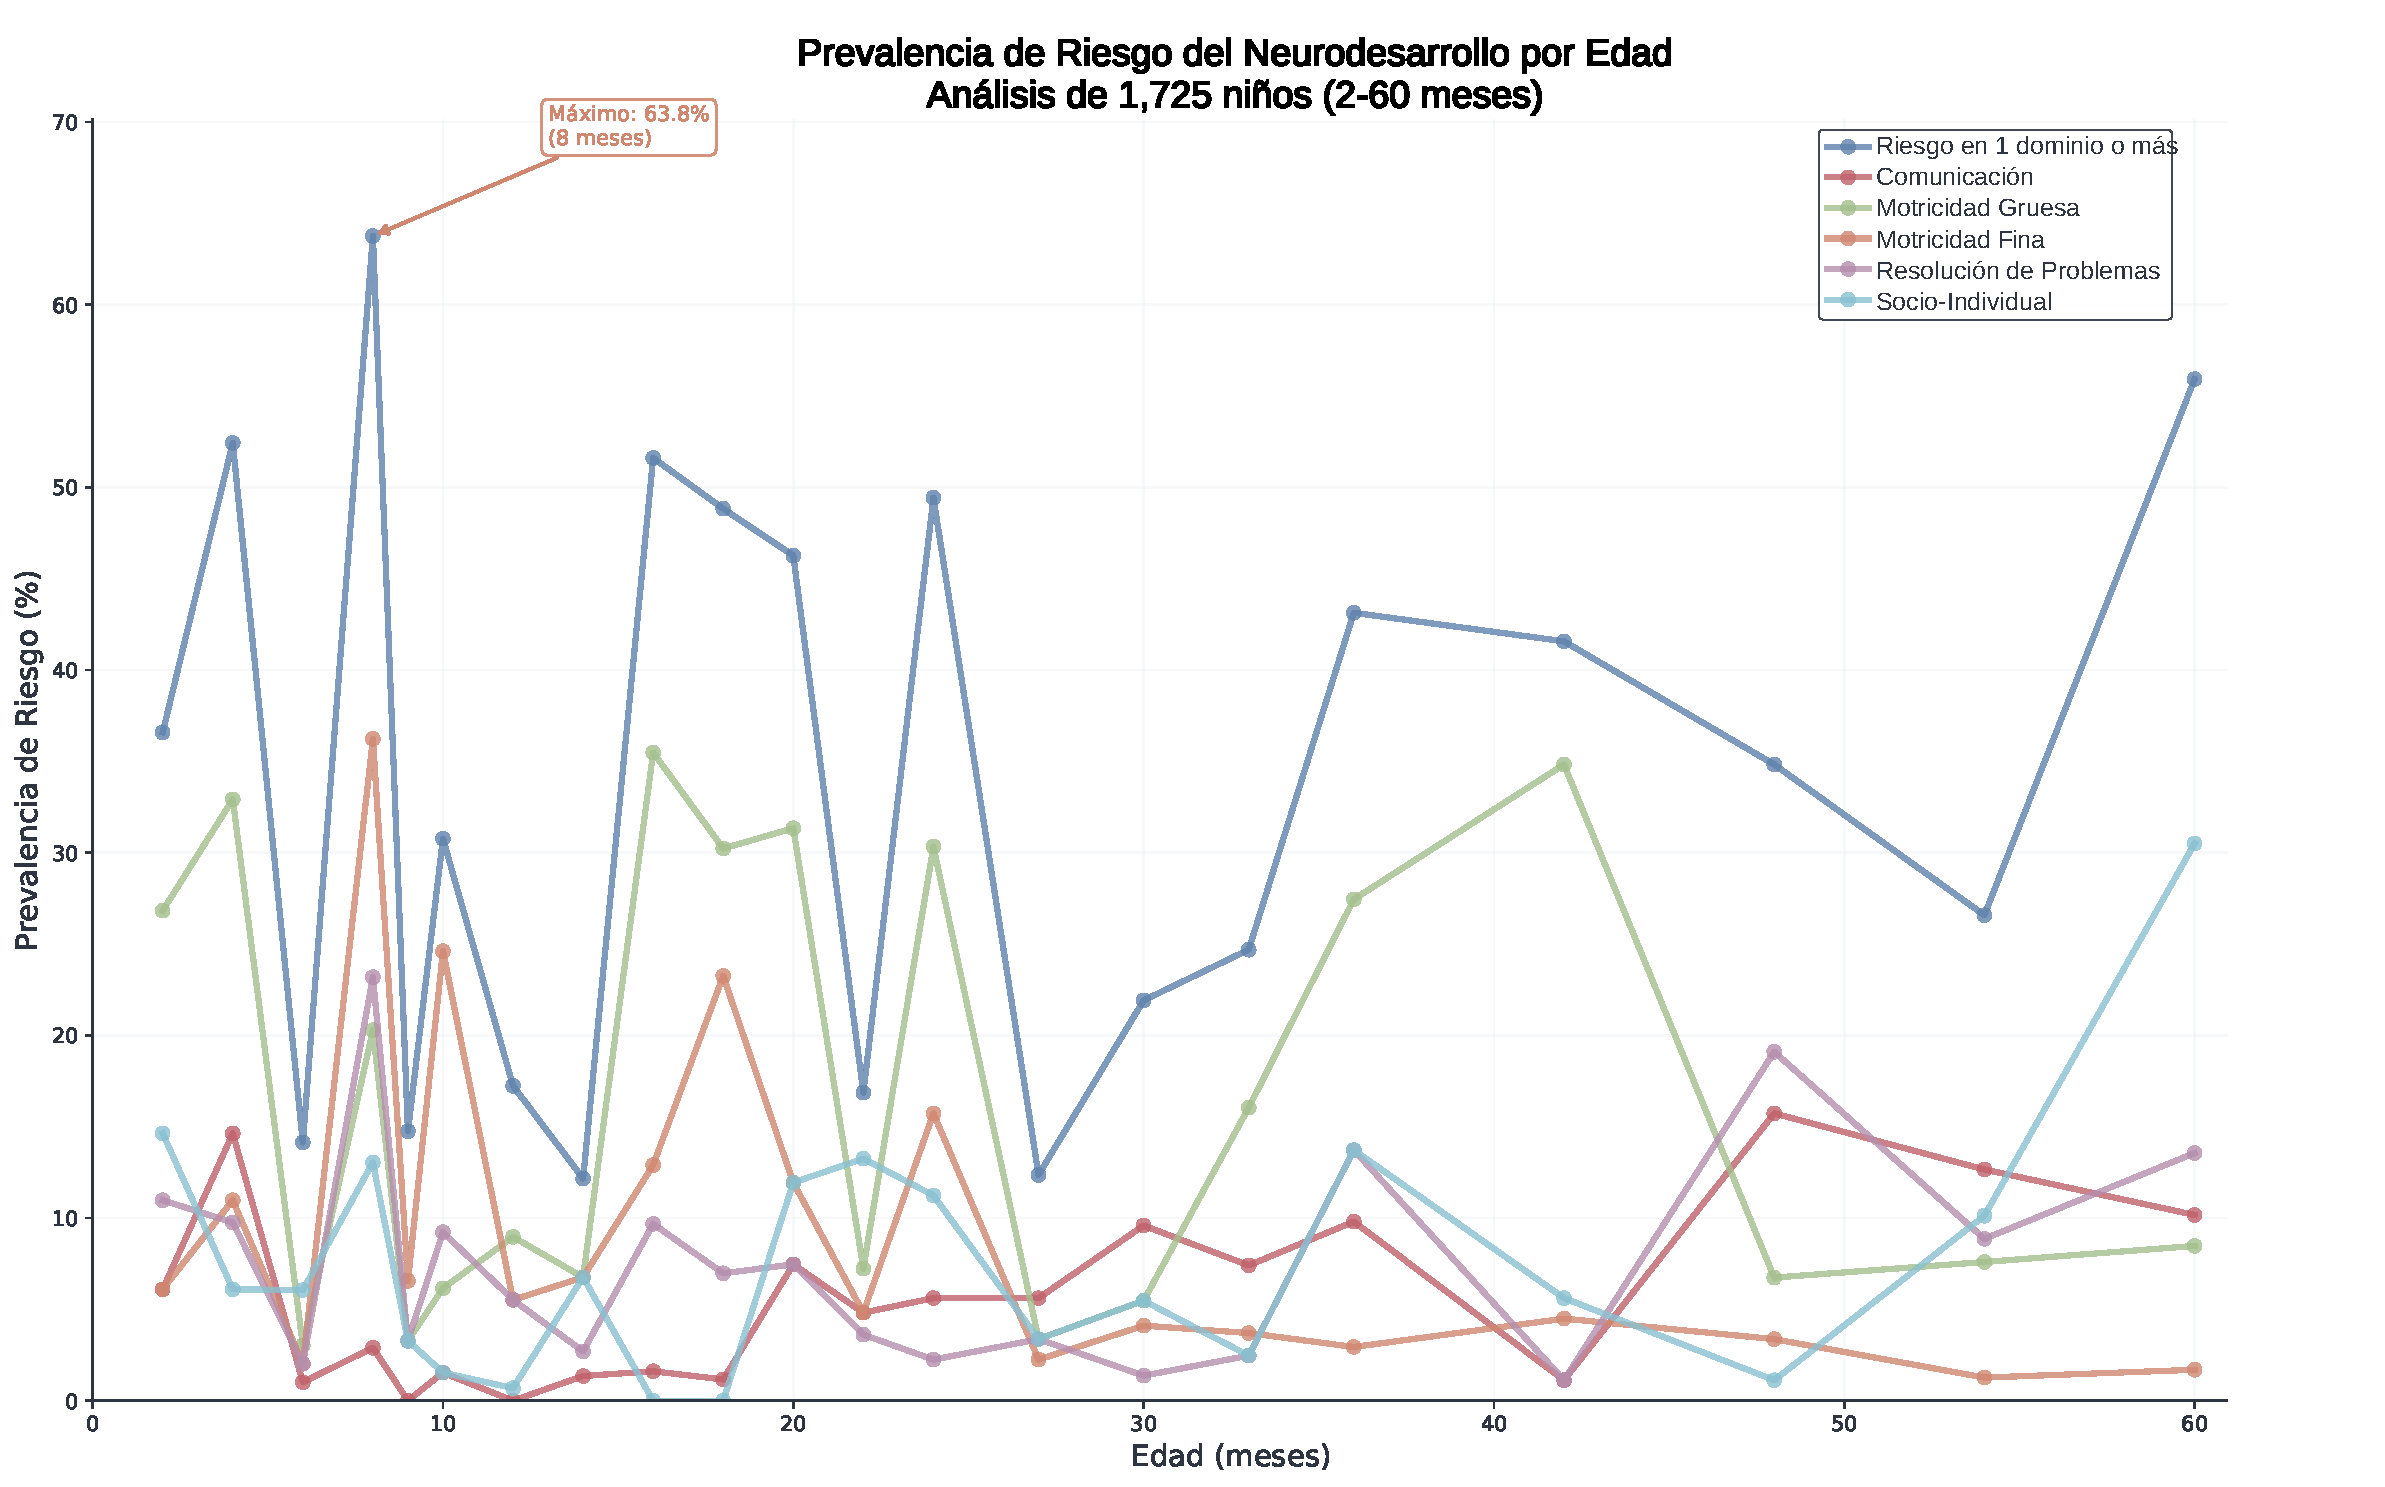
\includegraphics[width=1\textwidth]{prevalencia_edad_nord}
	\captionsetup{font=footnotesize}
	\caption{Prevalencia de riesgo en el desarrollo de acuerdo a rangos de edad
	del ASQ-3.}
    \label{fig:prevalencia_riesgo_asq3}
\end{figure}

\begin{figure}[htbp]
    \centering
    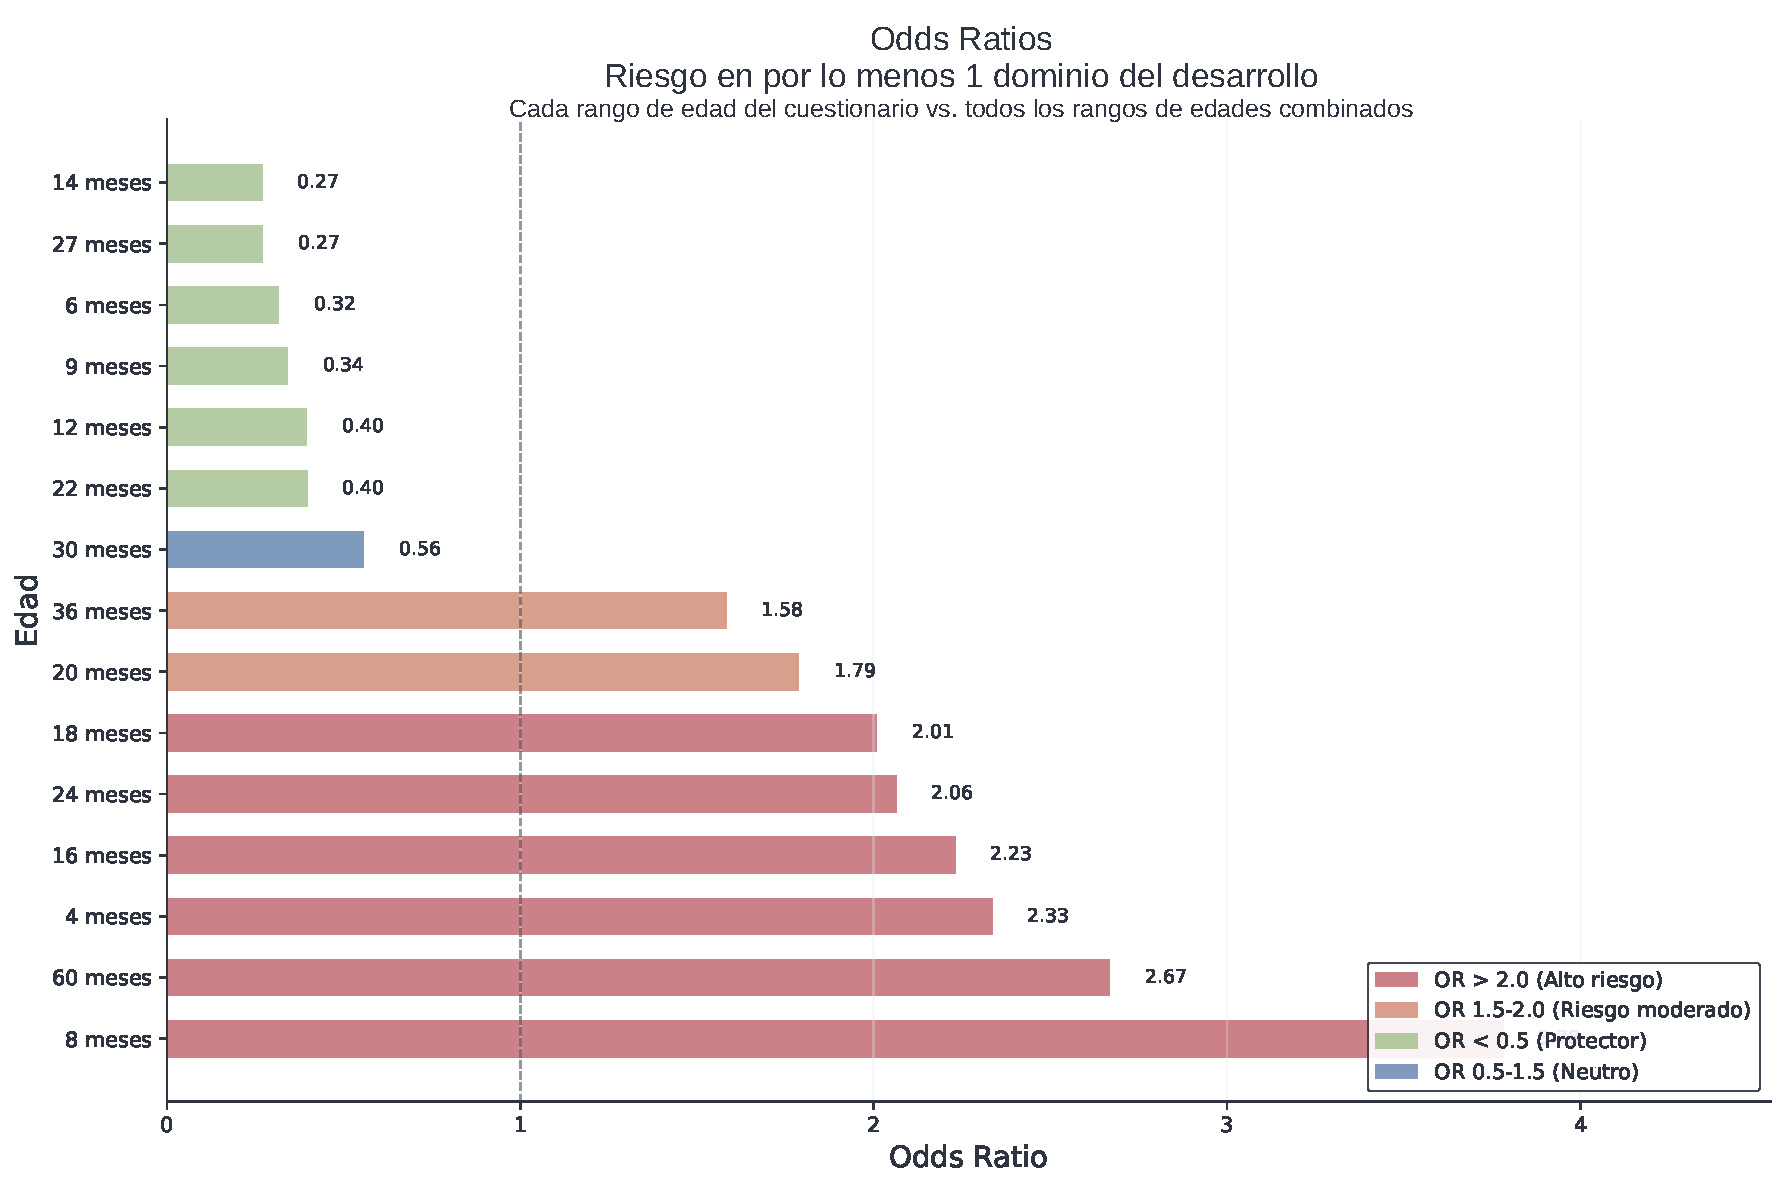
\includegraphics[width=1\textwidth]{odds_ratios_nord}
	\captionsetup{font=footnotesize}
	\caption{Odds ratio de presentar al menos 1 dominio en riesgo de acuerdo a
	los rangos de edades evaluados por los cuestionarios ASQ-3.}
    \label{fig:odds_ratio_asq3}
\end{figure}

\begin{table}[htbp]
\centering
\caption{Distribución y asociación de la variable \textit{sexo del niño} con los dominios del desarrollo}
\label{tab:sexo_nino_desarrollo_chi2}
\begin{threeparttable}
\begin{tblr}{
  width = \linewidth,
  colspec = {X[2,l]X[1,c]X[1,c]X[1,c]X[1,c]X[1,c]X[1,c]X[1,c]},
  row{1} = {font=\bfseries, bg=gray!10},
  row{even} = {bg=gray!3},
  cells = {valign=m, font=\footnotesize},
  hline{1,2,Z} = {1pt},
  hline{3-Y} = {0.5pt, gray},
}
\textbf{Dominio} & \textbf{Sexo} & \textbf{Desarrollo adecuado} & \textbf{En riesgo} & \textbf{Alto riesgo} & \textbf{Total} & $\chi^2$ & \textit{p}-valor \\
Comunicación          & Femenino    & 765 & 34  & 4  & 803 & 2.986 & 0.225 \\
                      & Masculino   & 863 & 49  & 10 & 922 &       &       \\
                      & \textbf{Total}      & \textbf{1628} & \textbf{83}  & \textbf{14} & \textbf{1725} &       &       \\
Motricidad gruesa     & Femenino    & 669 & 105 & 29 & 803 & 1.376 & 0.503 \\
                      & Masculino   & 768 & 129 & 25 & 922 &       &       \\
                      & \textbf{Total}      & \textbf{1437} & \textbf{234} & \textbf{54} & \textbf{1725} &       &       \\
Motricidad fina       & Femenino    & 741 & 51  & 11 & 803 & 1.591 & 0.451 \\
                      & Masculino   & 836 & 73  & 13 & 922 &       &       \\
                      & \textbf{Total}      & \textbf{1577} & \textbf{124} & \textbf{24} & \textbf{1725} &       &       \\
Resolución de problemas & Femenino  & 751 & 47  & 5  & 803 & 1.957 & 0.376 \\
                      & Masculino   & 846 & 69  & 7  & 922 &       &       \\
                      & \textbf{Total}      & \textbf{1597} & \textbf{116} & \textbf{12} & \textbf{1725} &       &       \\
Socio-individual      & Femenino    & 745 & 49  & 9  & 803 & 0.340 & 0.844 \\
                      & Masculino   & 855 & 59  & 8  & 922 &       &       \\
                      & \textbf{Total}      & \textbf{1600} & \textbf{108} & \textbf{17} & \textbf{1725} &       &       \\
\end{tblr}
\begin{tablenotes}
\footnotesize
\item \textbf{Método:} Prueba chi-cuadrado.
\item \textbf{Nota:} Todas las asociaciones entre sexo y dominio de desarrollo no fueron estadísticamente significativas (\textit{p} $>$ 0.05).
\end{tablenotes}
\end{threeparttable}
\end{table}

\begin{table}[htbp]
\centering
\caption{Asociación entre grupo étnico y riesgo en dominios del desarrollo}
\label{tab:grupo_etnico_desarrollo_chi2_compacta}
\begin{threeparttable}
\begin{tblr}{
  width = 0.75\linewidth,
  colspec = {X[1.5,l]X[1.0,c]X[1.1,c]X[1.0,c]X[1.3,c]X[1.1,c]},
  row{1} = {font=\bfseries, bg=gray!10},
  row{even} = {bg=gray!3},
  cells = {valign=m, font=\footnotesize},
  hline{1,2,Z} = {1pt},
  hline{3-Y} = {0.5pt, gray},
}
\textbf{Dominio} & \textbf{$\chi^2$} & \textbf{\textit{p}-valor} & \textbf{OR} & \textbf{IC 95\%} & \textbf{Significativo} \\
Comunicación          & 2.73   & 0.098     & --    & --            & No \\
Motricidad gruesa     & 0.39   & 0.533     & --    & --            & No \\
Motricidad fina       & 1.89   & 0.169     & --    & --            & No \\
Resolución de problemas & 4.57   & 0.033     & 1.50  & 1.05--2.16    & Sí \\
Socio-individual      & 4.90   & 0.027     & 1.53  & 1.06--2.21    & Sí \\
\end{tblr}
\begin{tablenotes}
\footnotesize
\item \textbf{Método:} Prueba chi-cuadrado.
\item \textbf{Interpretación:}
No se encontró asociación significativa en comunicación (OR no aplicable, $\chi^2$ = 2.73, \textit{p} = 0.098), motricidad gruesa (OR no aplicable, $\chi^2$ = 0.39, \textit{p} = 0.533) ni motricidad fina (OR no aplicable, $\chi^2$ = 1.89, \textit{p} = 0.169).
En resolución de problemas, el riesgo fue 1.50 veces mayor en el grupo indígena (OR = 1.50, IC 95\%: 1.05--2.16). En socio-individual, el riesgo fue 1.53 veces mayor en el grupo indígena (OR = 1.53, IC 95\%: 1.06--2.21).
\end{tablenotes}
\end{threeparttable}
\end{table}

\begin{table}[htbp]
\centering
\caption{Asociación entre área de residencia y riesgo en dominios del desarrollo}
\label{tab:area_residencia_desarrollo_chi2_compacta}
\begin{threeparttable}
\begin{tblr}{
  width = 0.75\linewidth,
  colspec = {X[1.5,l]X[1.0,c]X[1.1,c]X[1.0,c]X[1.3,c]X[1.1,c]},
  row{1} = {font=\bfseries, bg=gray!10},
  row{even} = {bg=gray!3},
  cells = {valign=m, font=\footnotesize},
  hline{1,2,Z} = {1pt},
  hline{3-Y} = {0.5pt, gray},
}
\textbf{Dominio} & \textbf{$\chi^2$} & \textbf{\textit{p}-valor} & \textbf{OR} & \textbf{IC 95\%} & \textbf{Significativo} \\
Comunicación          & 8.70   & 0.003     & 2.09  & 1.30--3.36    & Sí \\
Motricidad gruesa     & 12.62  & $<$0.001  & 1.79  & 1.31--2.46    & Sí \\
Motricidad fina       & 1.73   & 0.188     & --    & --            & No \\
Resolución de problemas & 25.13  & $<$0.001  & 2.77  & 1.85--4.15    & Sí \\
Socio-individual      & 15.06  & $<$0.001  & 2.31  & 1.52--3.51    & Sí \\
\end{tblr}
\begin{tablenotes}
\footnotesize
\item \textbf{Método:} Prueba chi-cuadrado.
\item \textbf{Nota:}
Se observó asociación significativa entre área de residencia y riesgo en comunicación (OR = 2.09, IC 95\%: 1.30--3.36), motricidad gruesa (OR = 1.79, IC 95\%: 1.31--2.46), resolución de problemas (OR = 2.77, IC 95\%: 1.85--4.15) y socio-individual (OR = 2.31, IC 95\%: 1.52--3.51) (\textit{p} $<$ 0.01). El riesgo de retraso fue mayor en el área rural.
En motricidad fina, no se encontró asociación significativa (OR no significativo, $\chi^2$ = 1.73, \textit{p} = 0.188).
\end{tablenotes}
\end{threeparttable}
\end{table}

\begin{table}[htbp]
\centering
\caption{Asociación entre estado civil del cuidador y riesgo en dominios del desarrollo}
\label{tab:estado_civil_cuidador_desarrollo}
\begin{threeparttable}
\begin{tblr}{
  width = 0.95\linewidth,
  colspec = {X[1.4,l]X[0.8,c]X[1.0,c]X[1.0,c]X[1.0,c]X[0.7,c]},
  row{1} = {font=\bfseries, bg=gray!10},
  row{even} = {bg=gray!3},
  cells = {valign=m, font=\footnotesize},
  hline{1,2,Z} = {1pt},
  hline{3-Y} = {0.5pt, gray},
}
\textbf{Dominio} & \textbf{F/W} & \textbf{\textit{p}-valor} & \textbf{Significativo} & \textbf{Método} & \textbf{N} \\
Comunicación          & 10.18   & $<$0.001  & Sí  & Welch's ANOVA & 1725 \\
Motricidad gruesa     & 5.03    & 0.007     & Sí  & ANOVA         & 1725 \\
Motricidad fina       & 1.60    & 0.202     & No  & ANOVA         & 1725 \\
Resolución de problemas & 6.12  & 0.002     & Sí  & Welch's ANOVA & 1725 \\
Socio-individual      & 3.88    & 0.021     & Sí  & ANOVA         & 1725 \\
\end{tblr}
\begin{tablenotes}
\footnotesize
\item \textbf{Nota}: Se observó asociación significativa en los dominios de
comunicación, motor gruesa, resolución de problemas y socio-individual. Los
niños de cuidadores solteros presentaron menores medias de puntajes Z en
dominios de comunicación, resolución de problemas y socio-individual;
cuidadores casados presentaron menores puntajes Z en motricidad gruesa.
El grupo de niños de cuidadores unidos presentaron mayores medias Z y menor
proporción de riesgo en comunicación, resolución de problemas y
socio-individual.
\end{tablenotes}
\end{threeparttable}
\end{table}

\begin{figure}[htbp]
    \centering
    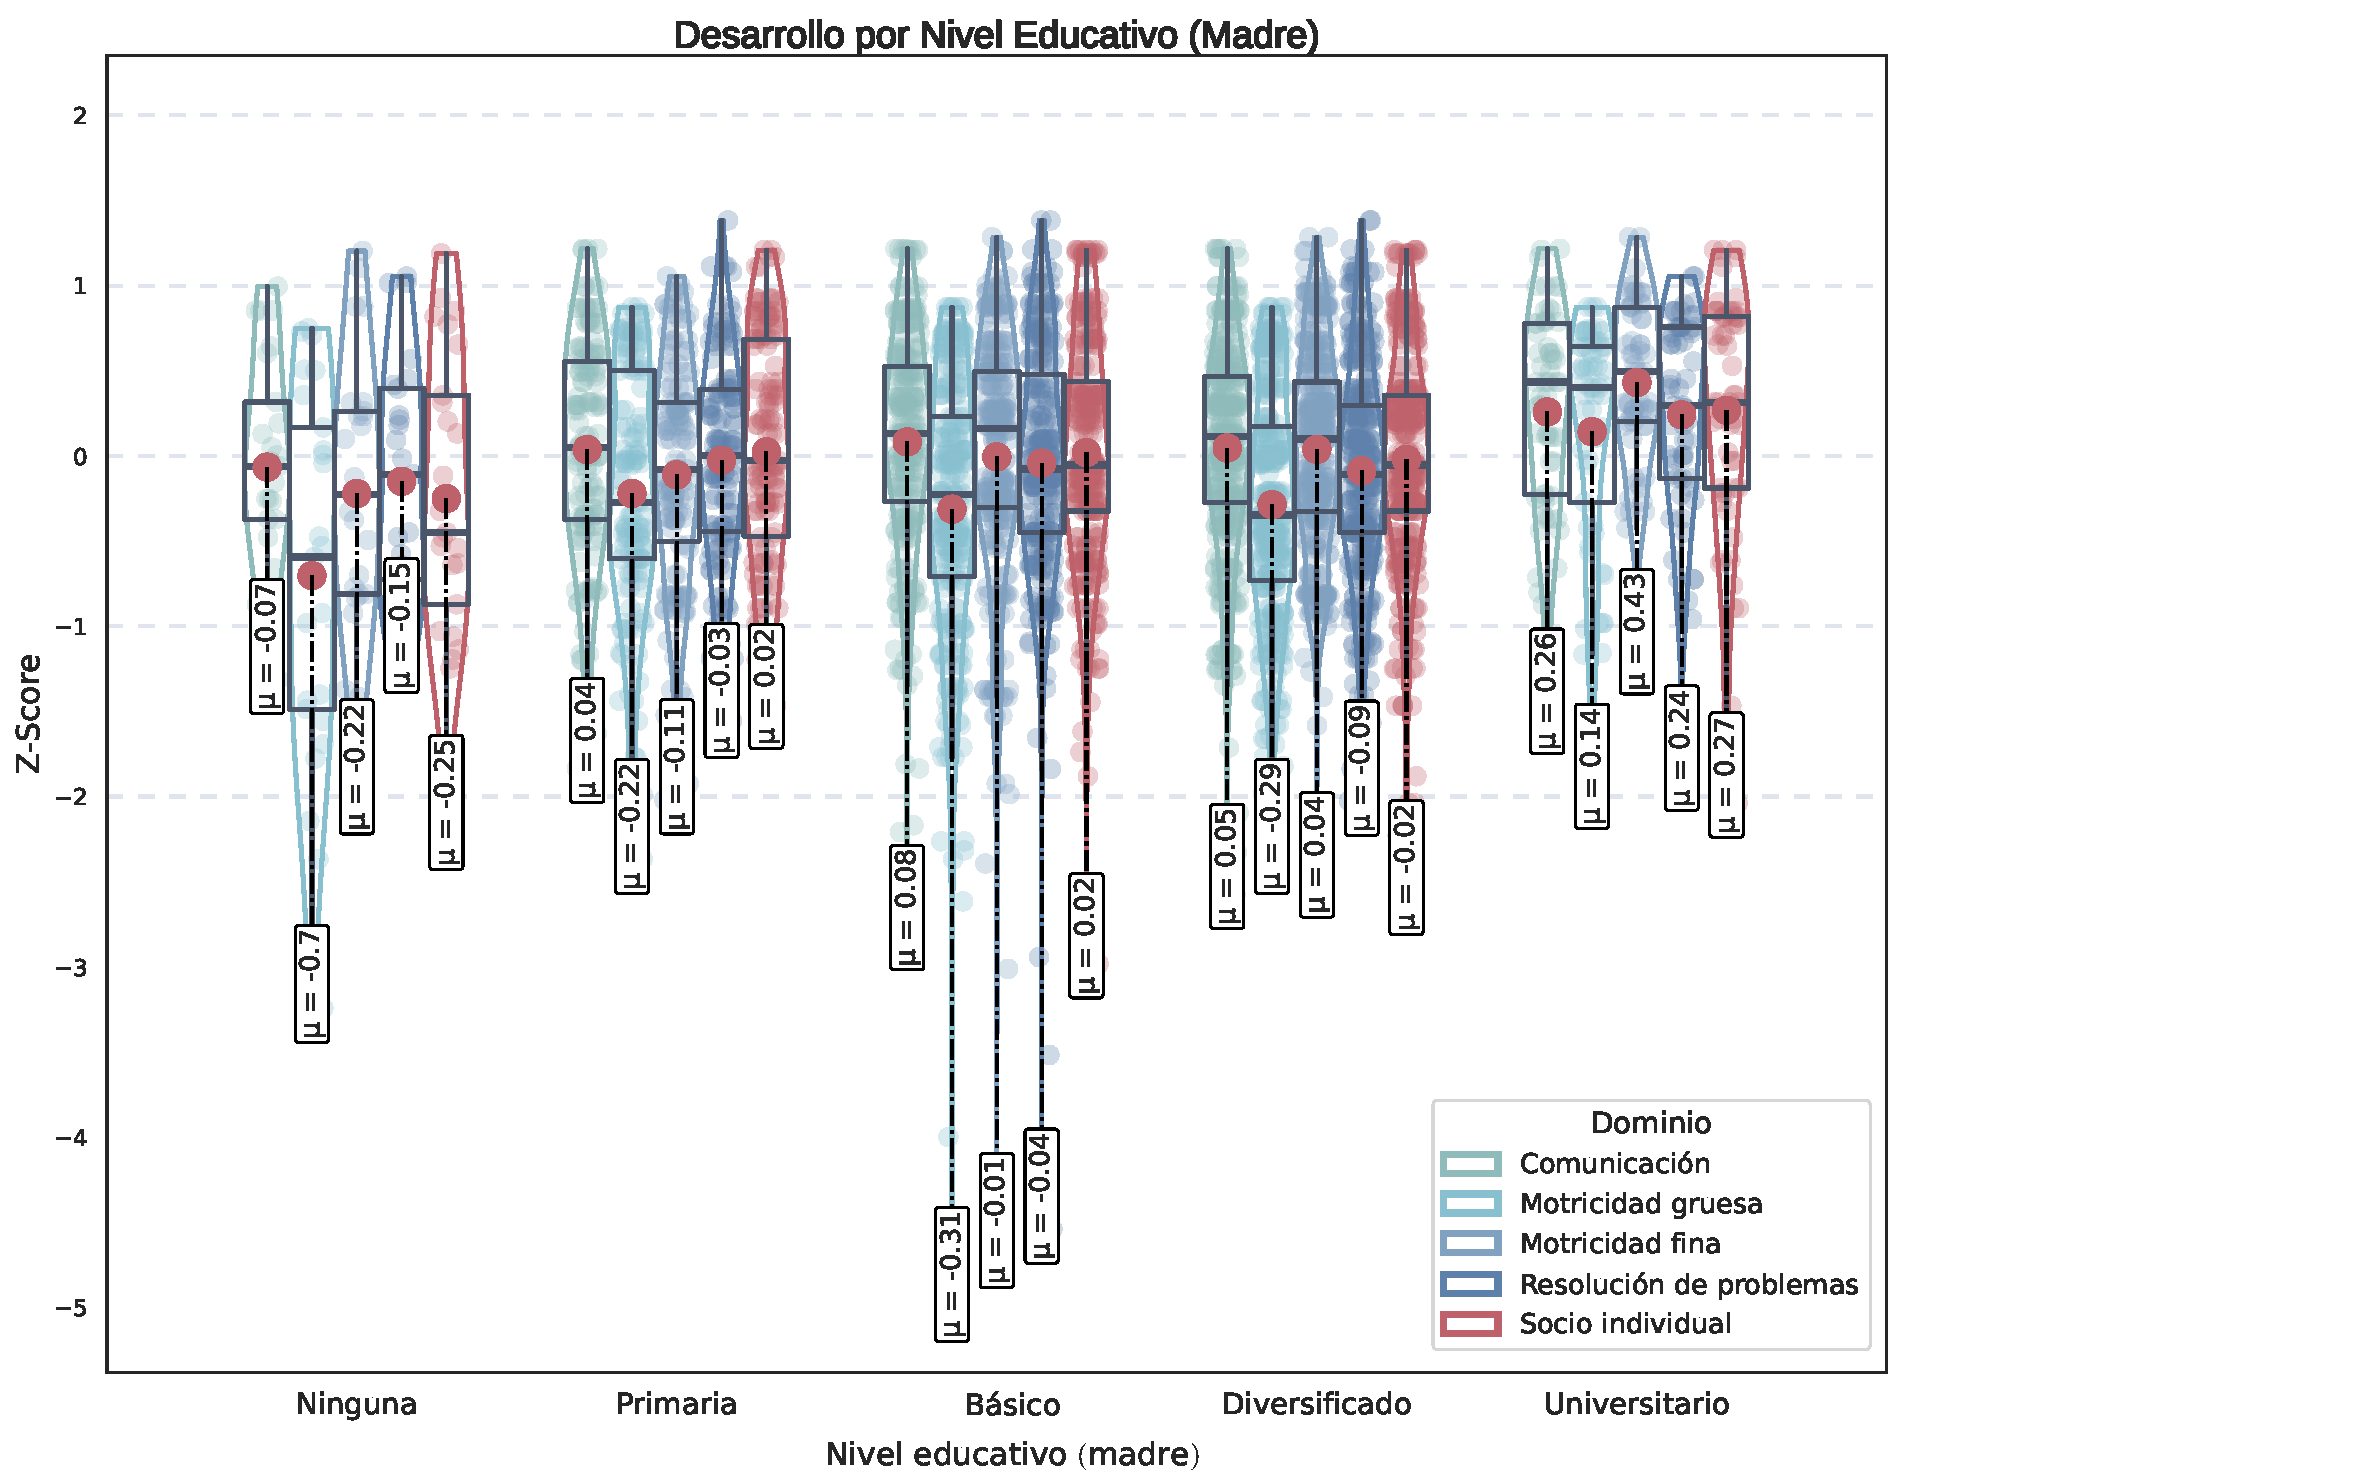
\includegraphics[width=1\textwidth]{violinplot_nivel_educativo_madre}
	\captionsetup{font=footnotesize}
	\caption{Desarrollo por nivel educativo (madre)}
    \label{fig:nivel_educativo_anova_madre}
\end{figure}

\begin{figure}[htbp]
    \centering
    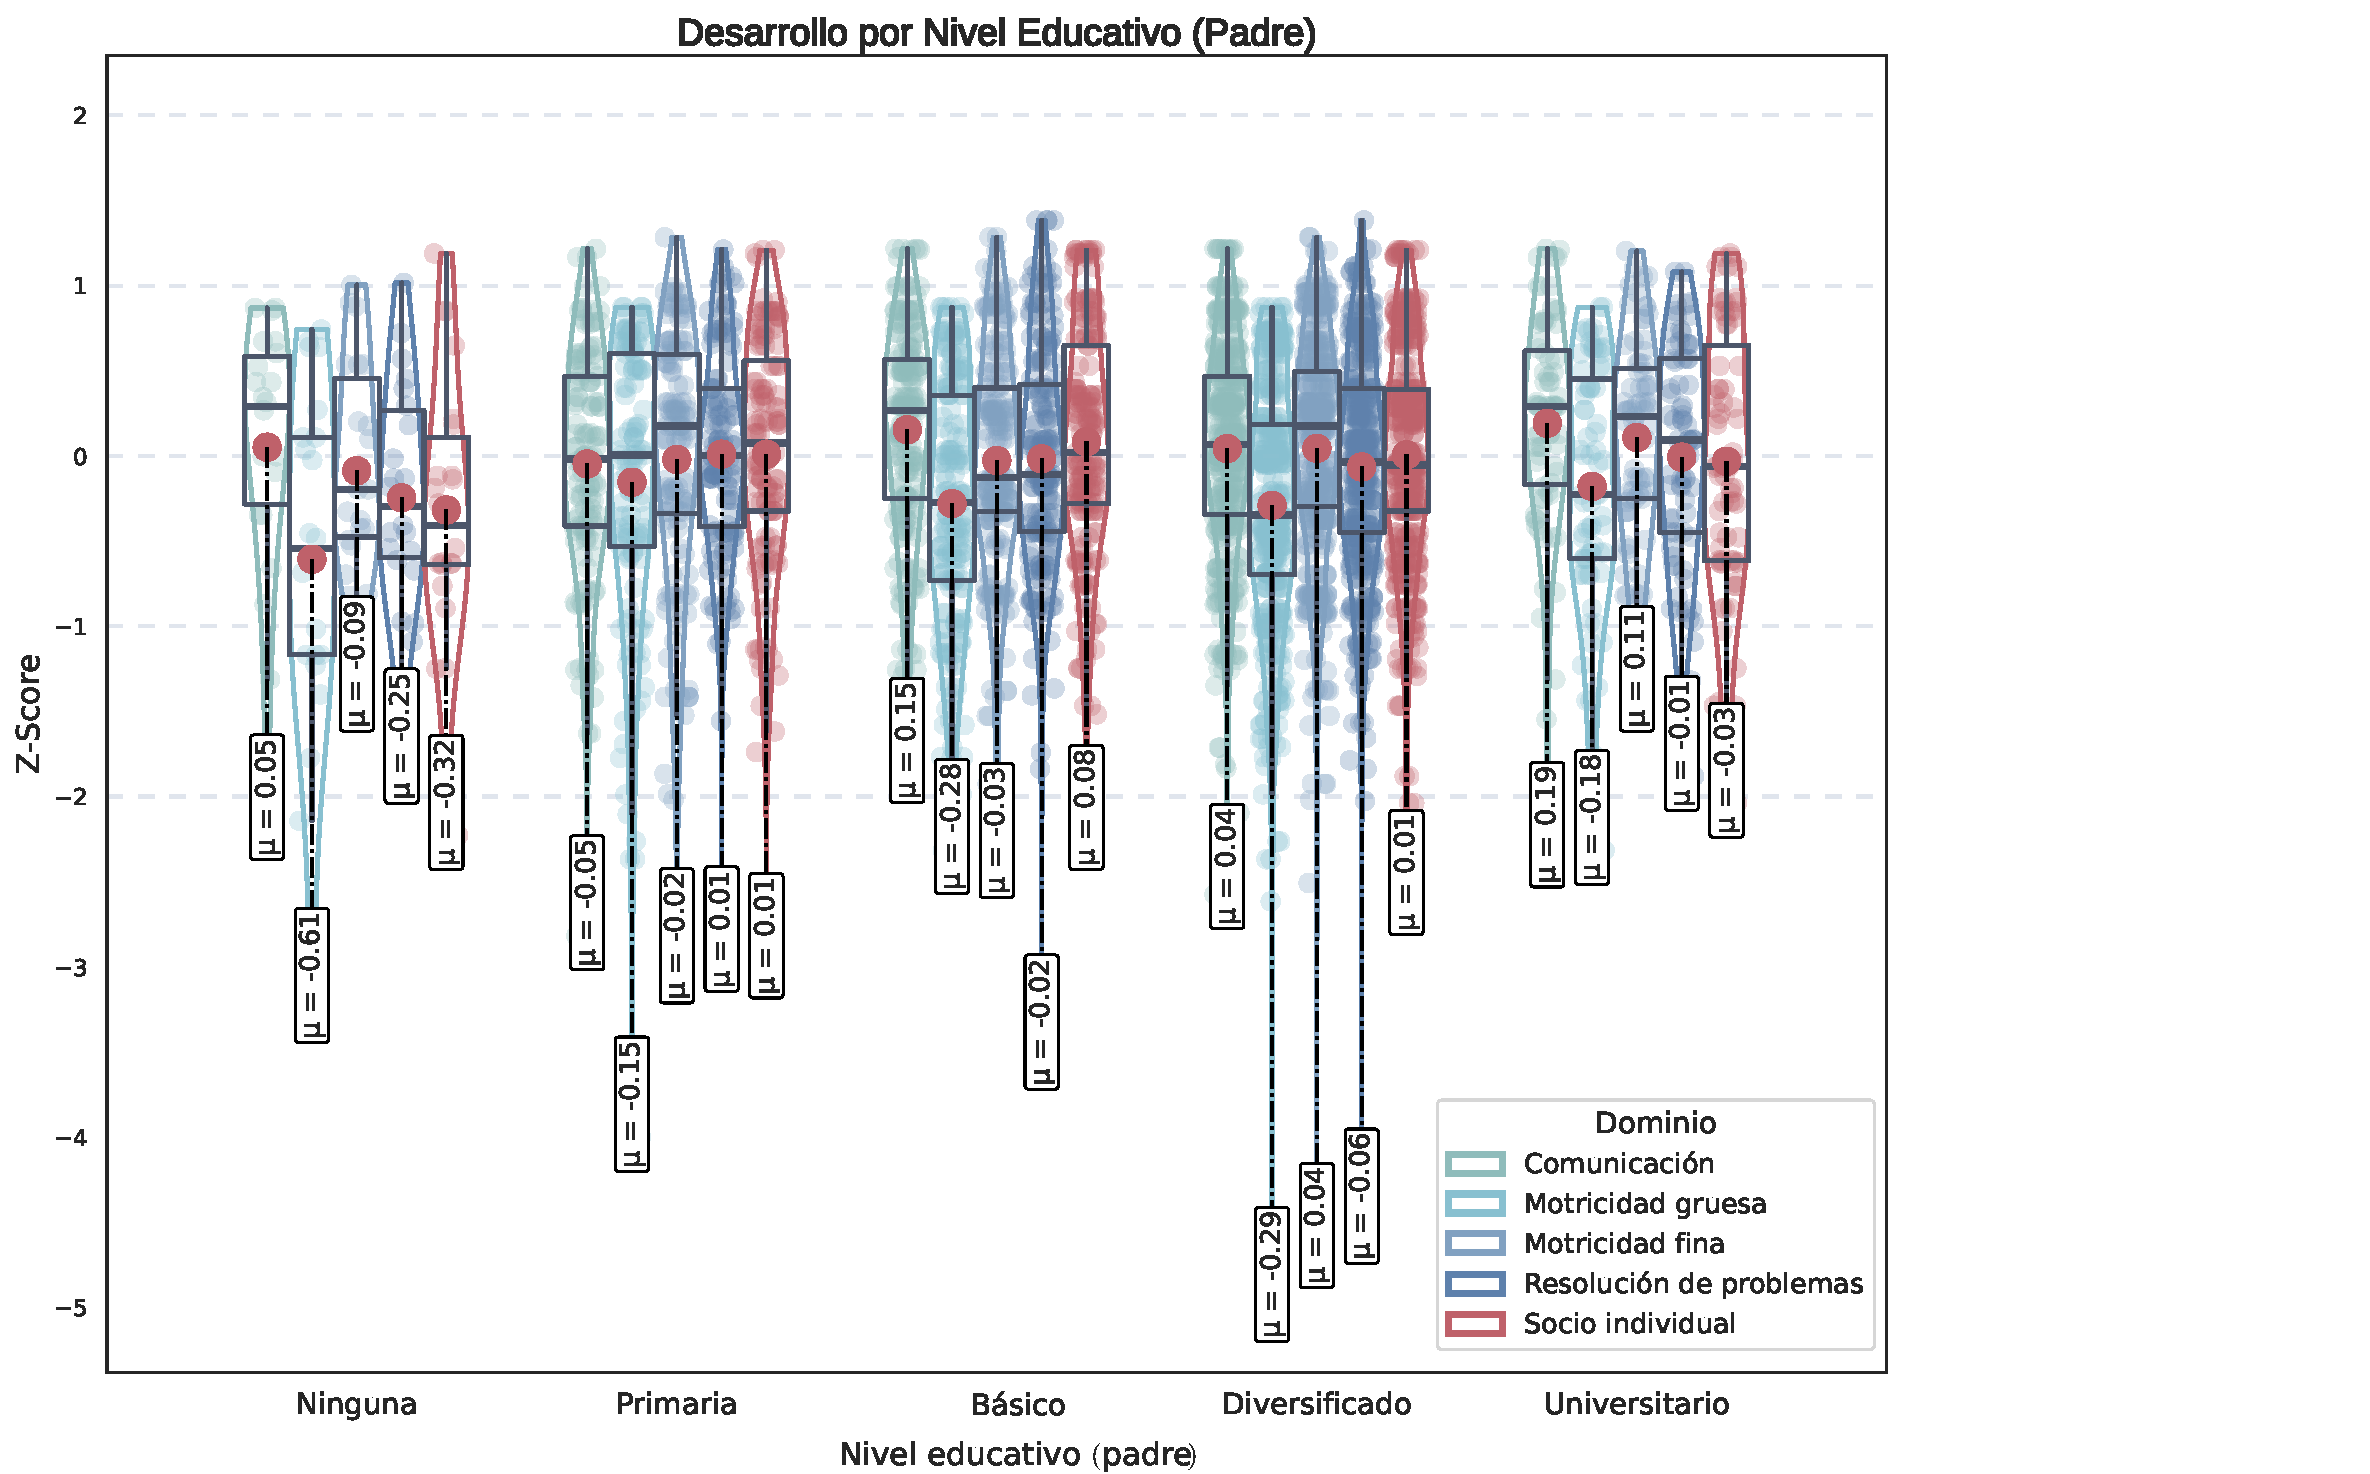
\includegraphics[width=1\textwidth]{violinplot_nivel_educativo_padre}
	\captionsetup{font=footnotesize}
	\caption{Desarrollo por nivel educativo (padre)}
    \label{fig:nivel_educativo_anova_padre}
\end{figure}

\begin{table}[htbp]
\centering
\caption{Asociación entre situación laboral del padre y riesgo en dominios del desarrollo}
\label{tab:situacion_laboral_padre_resumen_compacta}
\begin{threeparttable}
\begin{tblr}{
  width = 0.75\linewidth,
  colspec = {X[1.5,l]X[1.0,c]X[1.1,c]X[1.0,c]X[1.3,c]X[1.1,c]},
  row{1} = {font=\bfseries, bg=gray!10},
  row{even} = {bg=gray!3},
  cells = {valign=m, font=\footnotesize},
  hline{1,2,Z} = {1pt},
  hline{3-Y} = {0.5pt, gray},
}
\textbf{Dominio} & \textbf{$\chi^2$} & \textbf{\textit{p}-valor} & \textbf{OR} & \textbf{IC 95\%} & \textbf{Significativo} \\
Comunicación          & 0.57   & 0.451     & --    & --            & No \\
Motricidad gruesa     & 8.00   & 0.005     & 1.78  & 1.21--2.62    & Sí \\
Motricidad fina       & 0.51   & 0.473     & --    & --            & No \\
Resolución de problemas & 0.09   & 0.767     & --    & --            & No \\
Socio-individual      & 1.80   & 0.180     & --    & --            & No \\
\end{tblr}
\begin{tablenotes}
\footnotesize
\item \textbf{Método:} Prueba chi-cuadrado.
\item \textbf{Nota:} Dominios con asociaciones significativas: 1/5. El grupo de niños con padre que no trabaja tiene mayor riesgo en el dominio de motricidad gruesa (OR = 1.78).
\end{tablenotes}
\end{threeparttable}
\end{table}

\begin{table}[htbp]
\centering
\caption{Asociación entre el total de hermanos y riesgo en dominios del desarrollo}
\label{tab:total_hermanos_desarrollo}
\begin{threeparttable}
\begin{tblr}{
  width = 0.97\linewidth,
  colspec = {X[1.3,l]X[0.8,c]X[1.0,c]X[1.0,c]X[1.0,c]X[0.7,c]},
  row{1} = {font=\bfseries, bg=gray!10},
  row{even} = {bg=gray!3},
  cells = {valign=m, font=\footnotesize},
  hline{1,2,Z} = {1pt},
  hline{3-Y} = {0.5pt, gray},
}
\textbf{Dominio} & \textbf{F/W} & \textbf{\textit{p}-valor} & \textbf{Significativo} & \textbf{Método} & \textbf{N} \\
Comunicación          & 5.71   & $<$0.001  & Sí  & ANOVA         & 1725 \\
Motricidad gruesa     & 2.44   & 0.063     & No  & ANOVA         & 1725 \\
Motricidad fina       & 3.70   & 0.011     & Sí  & ANOVA         & 1725 \\
Resolución de problemas & 0.78 & 0.504     & No  & ANOVA         & 1725 \\
Socio-individual      & 2.91   & 0.034     & Sí  & ANOVA         & 1725 \\
\end{tblr}
\begin{tablenotes}
\footnotesize
\item \textbf{Nota:} En dominios de comunicación y socio-individual, el grupo de
>3 hermanos muestra mayor riesgo y menor desempeño en puntajes Z. En motricidad
fina, los grupos extremos (0 y >3 hermanos) presentan menor media Z que grupos
de 1 y 2 hermanos.
\end{tablenotes}
\end{threeparttable}
\end{table}

\begin{table}[htbp]
\centering
\caption{Asociación entre el orden al nacer del niño y riesgo en dominios del desarrollo}
\label{tab:posicion_hermanos_desarrollo}
\begin{threeparttable}
\begin{tblr}{
  width = 0.97\linewidth,
  colspec = {X[1.3,l]X[0.8,c]X[1.0,c]X[1.0,c]X[1.0,c]X[0.7,c]},
  row{1} = {font=\bfseries, bg=gray!10},
  row{even} = {bg=gray!3},
  cells = {valign=m, font=\footnotesize},
  hline{1,2,Z} = {1pt},
  hline{3-Y} = {0.5pt, gray},
}
\textbf{Dominio} & \textbf{F/W} & \textbf{\textit{p}-valor} & \textbf{Significativo} & \textbf{Método} & \textbf{N} \\
Comunicación          & 3.27   & 0.011     & Sí  & ANOVA         & 1725 \\
Motricidad gruesa     & 1.25   & 0.290     & No  & ANOVA         & 1725 \\
Motricidad fina       & 2.80   & 0.025     & Sí  & ANOVA         & 1725 \\
Resolución de problemas & 0.76 & 0.554     & No  & ANOVA         & 1725 \\
Socio-individual      & 0.73   & 0.571     & No  & ANOVA         & 1725 \\
\end{tblr}
\begin{tablenotes}
\footnotesize
\item \textbf{Nota:} El cuarto niño es el grupo más afectado en el dominio de
comunicación (mayor riesgo, menor media Z). El grupo de primogénitos es el que
presenta mayor riesgo en motricidad fina. El resto de dominios no presentan
resultados significativos.
\end{tablenotes}
\end{threeparttable}
\end{table}

\begin{table}[htbp]
\centering
\caption{Asociación entre tipo de parto y riesgo en dominios del desarrollo}
\label{tab:tipo_parto_desarrollo}
\begin{threeparttable}
\begin{tblr}{
  width = 0.85\linewidth,
  colspec = {X[1.4,l]X[0.8,c]X[1.0,c]X[1.0,c]X[1.0,c]X[0.7,c]},
  row{1} = {font=\bfseries, bg=gray!10},
  row{even} = {bg=gray!3},
  cells = {valign=m, font=\footnotesize},
  hline{1,2,Z} = {1pt},
  hline{3-Y} = {0.5pt, gray},
}
\textbf{Dominio} & \textbf{F/W} & \textbf{\textit{p}-valor} & \textbf{Significativo} & \textbf{Método} & \textbf{N} \\
Comunicación          & 2.26   & 0.106     & No  & Welch's ANOVA & 1725 \\
Motricidad gruesa     & 0.04   & 0.956     & No  & Welch's ANOVA & 1725 \\
Motricidad fina       & 0.77   & 0.462     & No  & ANOVA         & 1725 \\
Resolución de problemas & 0.19 & 0.828     & No  & Welch's ANOVA & 1725 \\
Socio-individual      & 0.82   & 0.439     & No  & Welch's ANOVA & 1725 \\
\end{tblr}
\begin{tablenotes}
\footnotesize
\item \textbf{Nota:} No se encontraron asociaciones significativas entre el tipo de parto y el riesgo en ningún dominio del desarrollo infantil (\textit{p} $>$ 0.05 en todos los casos).
\end{tablenotes}
\end{threeparttable}
\end{table}

\begin{table}[htbp]
\centering
\caption{Asociación entre servicio de asistencia al parto y riesgo en dominios del desarrollo}
\label{tab:servicio_asistencia_parto_desarrollo}
\begin{threeparttable}
\begin{tblr}{
  width = 0.85\linewidth,
  colspec = {X[1.4,l]X[0.8,c]X[1.0,c]X[1.0,c]X[1.0,c]X[0.7,c]},
  row{1} = {font=\bfseries, bg=gray!10},
  row{even} = {bg=gray!3},
  cells = {valign=m, font=\footnotesize},
  hline{1,2,Z} = {1pt},
  hline{3-Y} = {0.5pt, gray},
}
\textbf{Dominio} & \textbf{F/W} & \textbf{\textit{p}-valor} & \textbf{Significativo} & \textbf{Método} & \textbf{N} \\
Comunicación          & 1.65   & 0.159     & No  & ANOVA         & 1725 \\
Motricidad gruesa     & 1.32   & 0.262     & No  & ANOVA         & 1725 \\
Motricidad fina       & 0.69   & 0.598     & No  & ANOVA         & 1725 \\
Resolución de problemas & 0.73 & 0.570     & No  & ANOVA         & 1725 \\
Socio-individual      & 2.41   & 0.072     & No  & Welch's ANOVA & 1725 \\
\end{tblr}
\begin{tablenotes}
\footnotesize
\item \textbf{Nota:} No se encontraron asociaciones significativas entre el servicio de asistencia al parto y el riesgo en ningún dominio del desarrollo infantil (\textit{p} $>$ 0.05 en todos los casos).
\end{tablenotes}
\end{threeparttable}
\end{table}

\begin{table}[htbp]
\centering
\caption{Asociación entre antecedentes de retardo de crecimiento y riesgo en dominios del desarrollo}
\label{tab:retardo_crecimiento_chi2_compacta}
\begin{threeparttable}
\begin{tblr}{
  width = 0.75\linewidth,
  colspec = {X[1.5,l]X[1.0,c]X[1.1,c]X[1.0,c]X[1.3,c]X[1.1,c]},
  row{1} = {font=\bfseries, bg=gray!10},
  row{even} = {bg=gray!3},
  cells = {valign=m, font=\footnotesize},
  hline{1,2,Z} = {1pt},
  hline{3-Y} = {0.5pt, gray},
}
\textbf{Dominio} & \textbf{$\chi^2$} & \textbf{\textit{p}-valor} & \textbf{OR} & \textbf{IC 95\%} & \textbf{Significativo} \\
Comunicación          & 0.81   & 0.369     & --    & --            & No \\
Motricidad gruesa     & 4.60   & 0.032     & 0.66  & 0.46--0.95    & Sí \\
Motricidad fina       & 3.69   & 0.055     & --    & --            & No \\
Resolución de problemas & 0.43   & 0.510     & --    & --            & No \\
Socio-individual      & 8.01   & 0.005     & 0.49  & 0.31--0.79    & Sí \\
\end{tblr}
\begin{tablenotes}
\footnotesize
\item \textbf{Método:} Prueba chi-cuadrado.
\item \textbf{Nota:} El retardo de crecimiento afecta significativamente 2 de 5 dominios del neurodesarrollo, con mayor impacto en motricidad gruesa (OR = 0.66).
\end{tablenotes}
\end{threeparttable}
\end{table}

\begin{table}[htbp]
\centering
\caption{Asociación entre antecedente de desnutrición aguda y riesgo en dominios del desarrollo}
\label{tab:desnutricion_aguda_resumen_compacta}
\begin{threeparttable}
\begin{tblr}{
  width = 0.75\linewidth,
  colspec = {X[1.5,l]X[1.0,c]X[1.1,c]X[1.0,c]X[1.3,c]X[1.1,c]},
  row{1} = {font=\bfseries, bg=gray!10},
  row{even} = {bg=gray!3},
  cells = {valign=m, font=\footnotesize},
  hline{1,2,Z} = {1pt},
  hline{3-Y} = {0.5pt, gray},
}
\textbf{Dominio} & \textbf{$\chi^2$} & \textbf{\textit{p}-valor} & \textbf{OR} & \textbf{IC 95\%} & \textbf{Significativo} \\
Comunicación          & 1.50   & 0.221     & --    & --            & No \\
Motricidad gruesa     & 0.90   & 0.342     & --    & --            & No \\
Motricidad fina       & 1.00   & 0.316     & --    & --            & No \\
Resolución de problemas & 1.30   & 0.254     & --    & --            & No \\
Socio-individual      & 4.05   & 0.044     & 1.97  & 1.07--3.64    & Sí \\
\end{tblr}
\begin{tablenotes}
\footnotesize
\item \textbf{Método:} Prueba chi-cuadrado.
\item \textbf{Nota:} El antecedente de desnutrición aguda se asocia significativamente a riesgo en el dominio socio-individual (OR = 1.97).
\end{tablenotes}
\end{threeparttable}
\end{table}

\begin{table}[htbp]
\centering
\caption{Asociación entre hospitalización neonatal y riesgo en dominios del desarrollo}
\label{tab:hospitalizado_neonatal_resumen}
\begin{threeparttable}
\begin{tblr}{
  width = 0.8\linewidth,
  colspec = {X[1.5,l]X[1, c]X[1, c]X[1, c]X[1.2, c]X[1, c]},
  row{1} = {font=\bfseries, bg=gray!10},
  row{even} = {bg=gray!3},
  cells = {valign=m, font=\footnotesize},
  hline{1,2,Z} = {1pt},
  hline{3-Y} = {0.5pt, gray},
}
\textbf{Dominio} & \textbf{Chi-cuadrado} & \textbf{\textit{p}-valor} & \textbf{OR} & \textbf{IC 95\%} & \textbf{Significativo} \\
Comunicación          & 0.00  & 1.000  & -- & -- & No \\
Motricidad gruesa     & 1.39  & 0.238  & -- & -- & No \\
Motricidad fina       & 3.18  & 0.075  & -- & -- & No \\
Resolución de problemas & 0.79 & 0.375  & -- & -- & No \\
Socio-individual      & 2.47  & 0.116  & -- & -- & No \\
\end{tblr}
\begin{tablenotes}
\footnotesize
\item \textbf{Nota:} Esta variable no muestra asociaciones significativas con el
neurodesarrollo infantil en ningún dominio.
\end{tablenotes}
\end{threeparttable}
\end{table}

\begin{table}[htbp]
\centering
\caption{Asociación entre hospitalización en la infancia y riesgo en dominios del desarrollo}
\label{tab:hospitalizado_infancia_resumen}
\begin{threeparttable}
\begin{tblr}{
  width = 0.8\linewidth,
  colspec = {X[1.5,l]X[1, c]X[1, c]X[1, c]X[1.2, c]X[1, c]},
  row{1} = {font=\bfseries, bg=gray!10},
  row{even} = {bg=gray!3},
  cells = {valign=m, font=\footnotesize},
  hline{1,2,Z} = {1pt},
  hline{3-Y} = {0.5pt, gray},
}
\textbf{Dominio} & \textbf{Chi-cuadrado} & \textbf{\textit{p}-valor} & \textbf{OR} & \textbf{IC 95\%} & \textbf{Significativo} \\
Comunicación          & 0.44  & 0.509  & -- & -- & No \\
Motricidad gruesa     & 2.81  & 0.094  & -- & -- & No \\
Motricidad fina       & 1.46  & 0.227  & -- & -- & No \\
Resolución de problemas & 0.60 & 0.437  & -- & -- & No \\
Socio-individual      & 1.36  & 0.243  & -- & -- & No \\
\end{tblr}
\begin{tablenotes}
\footnotesize
\item \textbf{Nota:} Esta variable no muestra asociaciones significativas con el
neurodesarrollo infantil en ningún dominio.
\end{tablenotes}
\end{threeparttable}
\end{table}

\begin{table}[htbp]
\centering
\caption{Asociación entre las horas de exposición a pantallas y riesgo en dominios del desarrollo}
\label{tab:horas_exposicion_pantallas_desarrollo}
\begin{threeparttable}
\begin{tblr}{
  width = 0.97\linewidth,
  colspec = {X[1.3,l]X[0.8,c]X[1.0,c]X[1.0,c]X[1.0,c]X[0.7,c]},
  row{1} = {font=\bfseries, bg=gray!10},
  row{even} = {bg=gray!3},
  cells = {valign=m, font=\footnotesize},
  hline{1,2,Z} = {1pt},
  hline{3-Y} = {0.5pt, gray},
}
\textbf{Dominio} & \textbf{F/W} & \textbf{\textit{p}-valor} & \textbf{Significativo} & \textbf{Método} & \textbf{N} \\
Comunicación          & 3.79   & 0.010     & Sí  & ANOVA         & 1725 \\
Motricidad gruesa     & 2.62   & 0.049     & Sí  & ANOVA         & 1725 \\
Motricidad fina       & 2.99   & 0.030     & Sí  & ANOVA         & 1725 \\
Resolución de problemas & 3.75 & 0.011     & Sí  & ANOVA         & 1725 \\
Socio-individual      & 4.33   & 0.005     & Sí  & ANOVA         & 1725 \\
\end{tblr}
\begin{tablenotes}
\footnotesize
\item En todos los dominios, se observa una tendencia a mayor riesgo en el
desarrollo con mayor número de horas de exposición a pantallas. Los grupos más
afectados son los de $\geq$ 6 horas en motricidad fina y 4-5 horas en
socio-individual.
\end{tablenotes}
\end{threeparttable}
\end{table}

\begin{table}[htbp]
\centering
\caption{Asociación entre las horas de juego con cuidador y riesgo en dominios del desarrollo}
\label{tab:horas_juego_cuidador_desarrollo}
\begin{threeparttable}
\begin{tblr}{
  width = 0.97\linewidth,
  colspec = {X[1.3,l]X[0.8,c]X[1.0,c]X[1.0,c]X[1.0,c]X[0.7,c]},
  row{1} = {font=\bfseries, bg=gray!10},
  row{even} = {bg=gray!3},
  cells = {valign=m, font=\footnotesize},
  hline{1,2,Z} = {1pt},
  hline{3-Y} = {0.5pt, gray},
}
\textbf{Dominio} & \textbf{F/W} & \textbf{\textit{p}-valor} & \textbf{Significativo} & \textbf{Método} & \textbf{N} \\
Comunicación          & 1.19   & 0.314     & No  & Welch's ANOVA & 1725 \\
Motricidad gruesa     & 3.05   & 0.028     & Sí  & ANOVA         & 1725 \\
Motricidad fina       & 2.57   & 0.053     & No  & ANOVA         & 1725 \\
Resolución de problemas & 6.49 & $<$0.001  & Sí  & ANOVA         & 1725 \\
Socio-individual      & 0.23   & 0.878     & No  & ANOVA         & 1725 \\
\end{tblr}
\begin{tablenotes}
\footnotesize
\item \textbf{Nota:} El grupo con menos horas de juego (0-1 horas) es el más
afectado en motricidad gruesa y resolución de problemas, mostrando mayor riesgo
y menores puntuaciones Z.
\end{tablenotes}
\end{threeparttable}
\end{table}
